\documentclass[
    10pt, 
    a4paper, 
    % draft
    ]{article}

\usepackage{titlesec}

\titleformat{\part}
    [hang]
    {\LARGE\bfseries}
    {}
    {0pt}
    {   
    \clearpage
    \begin{figure}
        
\includegraphics[width = 0.25\linewidth]{logo/hlogo.png}
    \end{figure}
    \setcounter{section}{0}
    \raggedright
}
\titlespacing{\part}{0pt}{0pt}{10pt}

\makeatletter

% Define the function
\newcommand{\relatorio}[4]{%
    \part{#1}

    #2

    \bigskip

    \noindent\colorbox{black!10}{\begin{minipage}{\textwidth}
        \vspace{10pt}
        \begin{center}
            \begin{minipage}{0.95\textwidth}
                \textbf{Resumo}
                \par #3
            \end{minipage}
        \end{center}
        \vspace{1pt}
    \end{minipage}}

    \bigskip

    Palavras-chave: #4
}

\makeatother
\usepackage[
    a4paper,
    includehead,
]{geometry}

\usepackage[portuguese]{babel}

\usepackage{keyval}

\usepackage[color = {[gray]{0.94}}]{draftwatermark}
\SetWatermarkText{RASCUNHO}
\SetWatermarkScale{4}

\linespread{1.25}
\setcounter{tocdepth}{-1}

%DIAGRAMAS E GRÁFICOS ----
\usepackage{tikz}
\usetikzlibrary{fit, arrows,automata,positioning, calc, decorations.pathreplacing, calligraphy}
\usepackage[edges]{forest}

%EQUAÇÕES E TABELAS ----
\usepackage{amsmath, amssymb}
\usepackage[makeroom]{cancel}
\usepackage{booktabs}
\usepackage{siunitx}


% \usepackage[nopatch]{microtype}
\usepackage{csquotes}
% \usepackage{caption}
\usepackage{subcaption}
\usepackage{xcolor}
\usepackage{changepage}
\usepackage{float}
\usepackage{array} %tabela com coluna de tamanho definido

\usepackage{graphicx}

\usepackage{subfiles}

%Margins and Header/Footer
\geometry{a4paper,
  top=0.75in,
  bottom=1.5in,
  left=1in,
  right=1in,
  headheight=14.5pt, % the default is too short
  heightrounded, % avoids the need of a flexible baselineskip
} 

\usepackage{hyperref}
% \hypersetup{
%     colorlinks=true,
%     linkcolor=blue,
%     filecolor=magenta,      
%     urlcolor=blue,
%     }

\usepackage[
  style=authoryear,
]{biblatex}

\usepackage{lipsum}




\usepackage{pgfplots}
\pgfplotsset{compat=newest}
\usepgfplotslibrary{statistics}
\usepgfplotslibrary{fillbetween}
\usetikzlibrary{decorations.markings,decorations.pathmorphing}
\def\nsamples{100}

\pgfplotsset{
    standard/.style={
    axis line style = thick,
    enlargelimits,
    axis x line=middle,
    axis y line=middle,
    enlarge x limits=0.15,
    enlarge y limits=0.15,
    % every axis x label/.style={at={(current axis.right of origin)},anchor=north west},
    % every axis y label/.style={at={(current axis.above origin)},anchor=south east}
    }
}
\usepackage{fancyhdr, etoolbox}
\pagestyle{fancy}
\renewcommand{\headrulewidth}{0pt}

% \newcommand{\parttitle}{}
% \makeatletter
% \patchcmd{\@part}% <cmd>
%   {\markboth}% <search>
%   {\renewcommand{\parttitle}{#1}}% <replace>
%   {}{}% <success><failure>
% \makeatother

% \fancyhead[L]{\parttitle}    


\addbibresource{citacoes.bib}
% \addbibresource{relatiorios/passe-livre/citacoes.bib}
% \addbibresource{relatiorios/macro/citacoes.bib}

%-----------------------------------------------------------------

\begin{document}

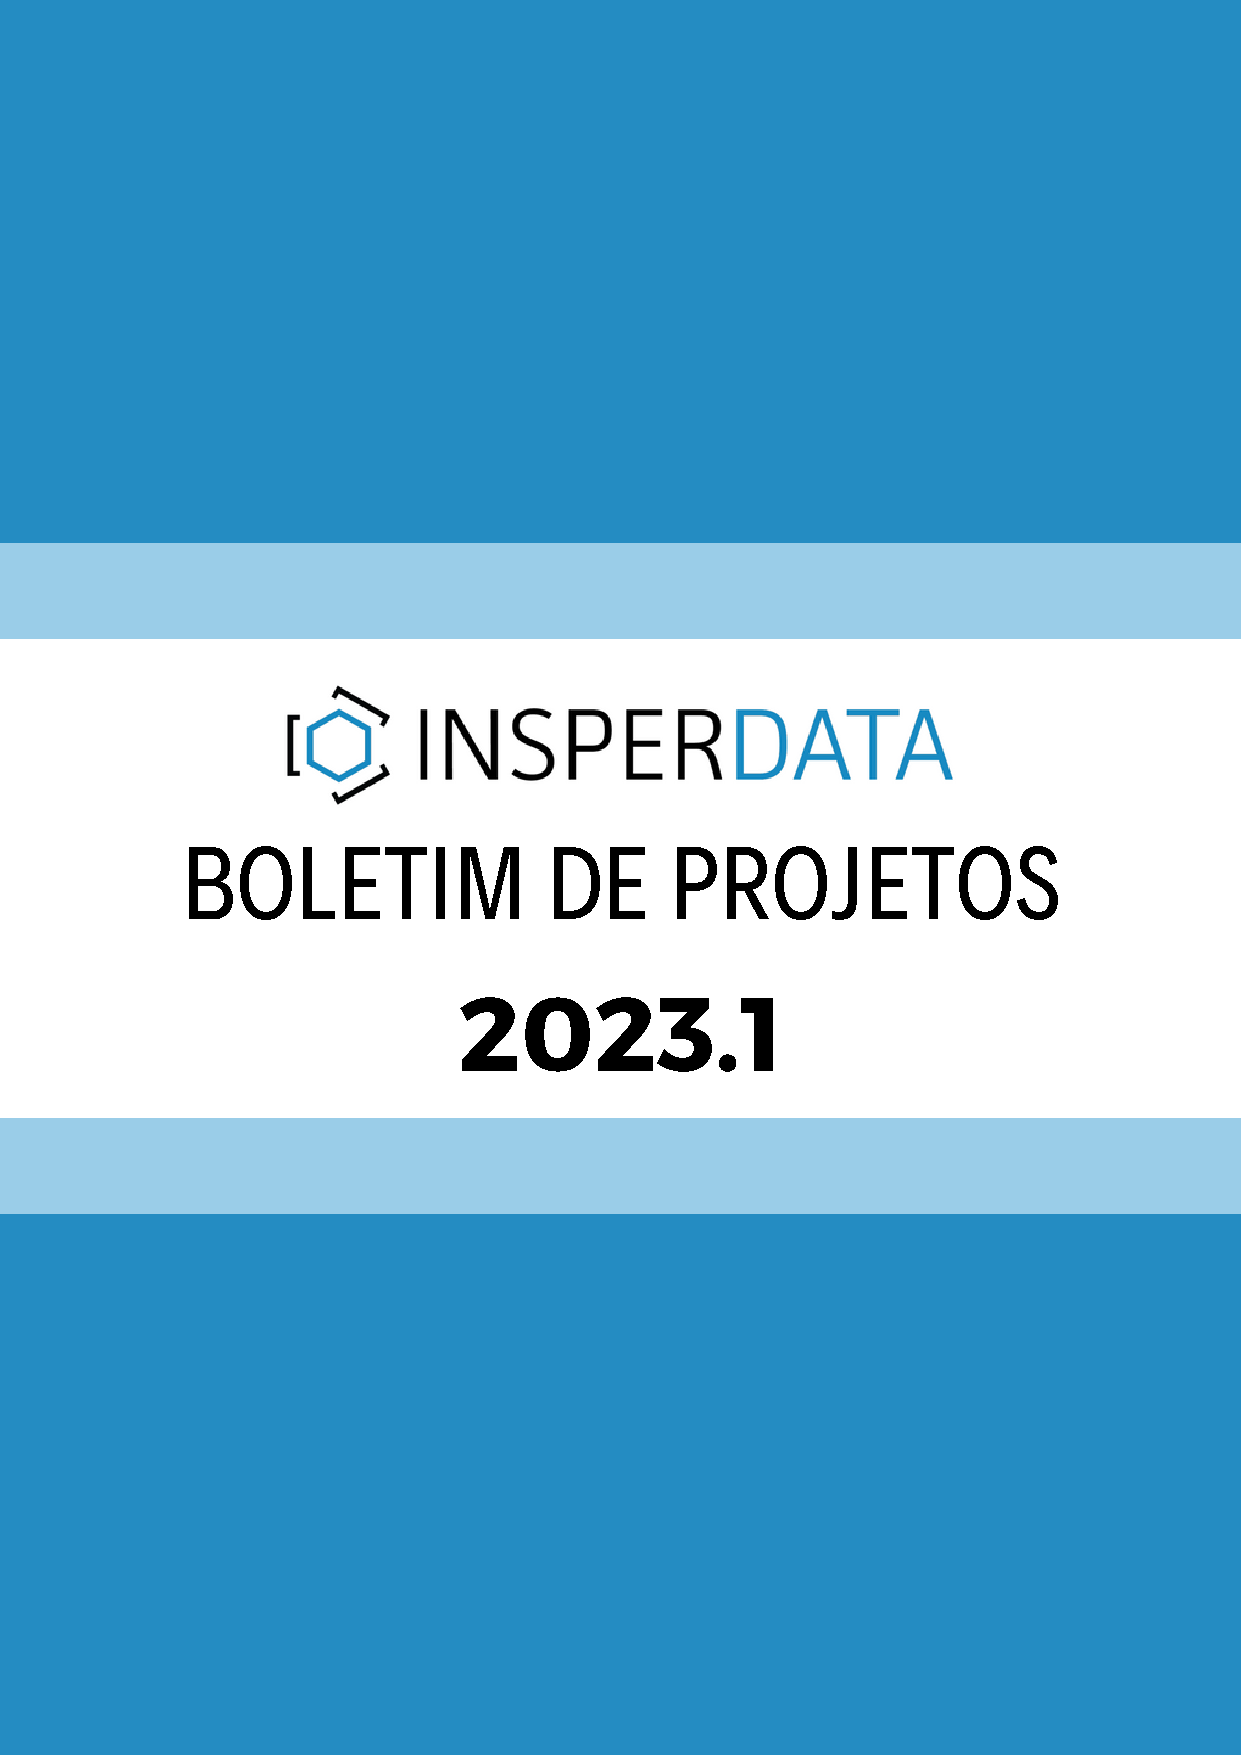
\includepdf[pages=-]{capa/capa.pdf}

\tableofcontents

\bigskip\bigskip

\noindent\rule{\linewidth}{.5pt}
\section*{Carta ao leitor}

Caro leitor,
com muita satisfação, o Insper Data convida todos a conheceremos projetos desenvolvidos durante o semestre.
Em primeiro lugar, o Insper Data é uma organização estudantil focada em pesquisa e ciência dos dados. Nosso propósito é garantir o desenvolvimento de forte capacidade analítica e de execução em uma entidade que preza pela excelência e contínuo aprendizado, utilizando métodos econômicos, matemáticos e estatísticos para resolver problemas reais.

Caminhamos nessa direção através da realização de projetos semestrais, nos quais os grupos escolhem tanto tema quanto orientador, que pode ser alguém com expertise acadêmica ou corporativa depender do escopo estudado. No semestre de 2023.1, foram confeccionados 6 trabalhos, abarcando as grandes áreas da microeconomia, macroeconomia, finanças, direito e modelagem preditiva. Além disso, neste semestre foram desenvolvidos os primeiros projetos de consultoria formal da entidade, área que tende a crescer dentro da organização. 

Embora com escopos e objetivos largamente distintos, todos os projetos desenvolvidos compartilham um denominador comum: a utilização de ciência dos dados como base para encontrar evidências empíricas acerca dos temas estudados. Desejamos a todos uma boa leitura!

\section{Introdução}

Nas eleições brasileiras de 2022, houve um grande movimento conhecido como Passe Livre pela Democracia, que lutou pela adoção do transporte público gratuito no dia da votação, para que mais pessoas votassem. O movimento enfrentou bastante resistência política e foi grande alvo de discussão. 

Essa medida tem seu mérito divido em dois aspectos, o primeiro deles sendo normativo, considerando a mobilidade como um direito e a dificuldade de uma pessoa se locomover à urna como uma possível barreira monetária ao exercício democrático de votar. O segundo aspecto se refere aos incentivos econômicos do voto, sendo que um estímulo monetário influencia a decisão das pessoas e pode ser decisivo para ``convencer'' um cidadão a votar.

Entretanto, esta medida pode ser um tanto quanto custosa e não há garantias de que as pessoas que usufruem do passe livre efetivamente estão aproveitando a medida para votar ou para realizar outras atividades. \textcite{pereira2023transporte} conduzem um estudo na tentativa de identificar essa hipótese, e seus resultados serão discutidos no tópico \ref{subsec_revisao}. Ademais, o conturbado cenário político complicou a execução da medida, visto que a comunicação dos governos municipais pode não ter sido eficiente e possivelmente a população não estava plenamente ciente da adoção do passe livre. 

O objetivo deste estudo é identificar se a adoção do passe livre causa uma redução na abstenção. Na seção \ref{sec_teor} é discutido o que é estabelecido na teoria de ciência política com um olhar microeconômico, bem como é feita uma adaptação dos modelos da literatura para o caso do passe livre. Na seção \ref{sec_modEmp} é feita uma tentativa empírica de medir o efeito do passe livre a partir de um \textit{diff-in-diff} pareado com efeitos fixos e um \textit{event study} para testes de robustez.

\section{Modelagem Teórica}
\label{sec_teor}

\subsection{Revisão Literária}
\label{subsec_revisLit}

A discussão sobre abstenção é extensiva no campo da economia política e diversos autores contribuíram com o debate de seus determinantes. \textcite{downs1957economic} é um dos precursores do modelo microeconômico que é continuado por uma série de autores. Sua premissa é simples: os eleitores buscam maximizar suas utilidades, que são definidas pela Equação \ref{eq_downs}. A partir disso, é considerado racional o eleitor que vota quando sua utilidade esperada é maior que zero e, caso contrário, se abstém. 

\begin{equation}
\label{eq_downs}
    \mathbb{E}(U_i)=B\cdot P-C
\end{equation}

Na equação, $\mathbb{E}(U_i)$ representa a utilidade esperada do cidadão $i$ apto, ao votar. Esta utilidade é impactada negativamente por $C$, o custo de votar, que se refere aos dispêndios de tempo, recursos e custos de oportunidade. Exemplos de fatores que podem afetar o custo são longas distâncias até as urnas, filas e demora para votar, o custo financeiro do transporte, fortes chuvas, etc. Os custos de não votar, como a necessidade de justificar o voto e pagar uma multa no caso brasileiro, são considerados nesse custo também afetando positivamente a utilidade de votar. A variável $B$ representa o benefício líquido de seu candidato favorito, caso seja eleito. Na análise de Downs, o benefício é dado por quanto o eleitor julga que sua primeira opção de candidato (A) seja melhor que a segunda opção (B), caso seja eleita: $B_{it} = \mathbb{E}(U^A_{t+1})-\mathbb{E}(U^B_{t+1})$. $P$ representa a probabilidade de seu voto ser decisivo. O voto decisivo é considerado aquele que desempata o resultado da eleição, caso o número de votantes seja ímpar, ou defina o resultado da votação, caso seja par. Em termos práticos, o benefício do candidato preferido apenas será importante para o eleitor, caso o seu voto seja a causa dele ser eleito.

O modelo apresenta uma série de complicações, que são inclusive discutidas de forma descritiva por Downs. Um eleitor indiferente entre os candidatos neste modelo apresenta benefício zero e não votaria para qualquer valor de $C$ positivo, então não seria racional votar branco. Além disso, em eleições de grande escala, como é o caso das eleições federais que apresentam mais de 150 milhões de votantes, a probabilidade do voto ser decisivo é muito próxima a zero. Nesses casos, caso o custo seja positivo, a utilidade do voto seria sempre negativa e ninguém votaria.

Para endereçar estes problemas, \textcite{riker1968theory} introduzem, entre outras contribuições, mais um componente autônomo da utilidade
\footnote{É considerado um componente autônomo aquele que não está relacionado à abstenção. Considerando que a probabilidade do voto ser decisivo é dada por $P = 1/v$, no qual v é o número de votantes, quanto maior for a abstenção, maior é a probabilidade do voto ser decisivo}
$D$. Este se refere ao dever cívico de votar, que não está relacionado à probabilidade do voto ser decisivo. O autor argumenta que há um ganho de utilidade ao contribuir com o sistema democrático, bem como pode haver o sentimento de arrependimento caso o sujeito se abstenha. Além disso, considera votar um ato político, relacionado à tradição. Por outro lado, reconhece que para a maior parte das pessoas $D<C$ e, portanto, ainda não seria racional votar em grandes eleições.

\begin{equation}
\label{eq_riker}
    \mathbb{E}(U_i)=B\cdot P-C+D
\end{equation}

Os pesquisadores da escolha racional geralmente são muito focados no interesse individual das escolhas, mas no final do século XX uma série de estudos e experimentos passaram a questionar e contribuir com evidências de comportamentos racionalmente altruístas. Alguns modelos de escolha racional foram revisitados e \textcite{fowler2006altruism} e \textcite{edlin2007voting} são autores que incorporam este componente no modelo de forma a dividir o benefício líquido em duas partes (Equação \ref{eq_fowler}). A variável $B_p$ se refere ao benefício líquido que o candidato proporciona ao indivíduo, enquanto $B_s$ se refere ao benefício social. A questão é que enquanto $B_p$ beneficia apenas o sujeito, $B_s$ beneficia a todos no país na visão do eleitor, então este benefício é multiplicado pela população $N$. Entretanto, o benefício social não necessariamente apresenta a mesma relevância ao eleitor, se comparado ao individual e $\alpha$ controla por este fator, de forma que para a maioria das pessoas $0<\alpha < 1$.

\begin{equation}
\label{eq_fowler}
    B_i = B_p + \alpha\cdot NB_s
\end{equation}

Outra contribuição de \textcite{edlin2007voting} foi de consolidar o que se considera a probabilidade do voto ser decisivo (Equação \ref{e1_edlin}). O coeficiente $K$ representa o grau de competitividade da eleição e quanto mais próximas forem os votos do candidato A em relação ao B, maior é a probabilidade do voto ser decisivo. Em uma votação em que a diferença de votos entre os candidatos está em torno de $10p.p$., $K=5$, enquanto uma diferença de $\pm 2p.p.$ resulta em um $K=25$. Portanto, a probabilidade do voto ser decisivo $P$ é dada pela competitividade dividida pelo número de votantes, que equivale ao total de eleitores elegíveis $E$ vezes taxa de comparecimento $t$.

\begin{equation}
\label{e1_edlin}
\begin{aligned}
    K &= \frac{1}{\log(V_A)-\log(V_B)}\\
    P &= K/(tE)
\end{aligned}
\end{equation}

Ao substituir as equações \ref{eq_fowler} e \ref{e1_edlin} em \ref{eq_riker}, têm-se a equação em sua forma final (Equação \ref{eq_final}). É interessante observar que na medida em que o número de votantes $V$ aumenta, o benefício pessoal se aproxima a zero, enquanto o benefício social não, pois quando o número de votantes aumenta, o número de pessoas beneficiadas $N$ também aumenta. Considerando os fatores agregados, as ideias primordiais de \textcite{downs1957economic} tornam-se mais robustas, mas o esqueleto se mantém igual: $\alpha NB_s$ representam o benefício líquido do voto, $\frac{K}{tE}$ é a probabilidade do voto ser decisivo e $C+D$ é o componente autônomo do voto.

\begin{equation}
\label{eq_final}
\begin{aligned}
    \mathbb{E}(U_i)&=(B_p + \alpha\cdot NB_s)\cdot \frac{K}{tE}-C+D\\
    &=\left(\cancel{\frac{B_p}{V}} + \frac{\alpha\cdot NB_s}{tE}\right)\cdot K-C+D\\
    &=\underbrace{\frac{\alpha NB_s}{1}}_B\cdot\underbrace{\frac{K}{tE}}_P-\underbrace{C+D}_A
\end{aligned}
\end{equation}

Um desdobramento peculiar desse modelo é uma espécie de paradoxo, que inclusive foi discutido por \textcite{downs1957economic}. Nessa relação paradoxal, quanto maior é a utilidade de votar $\uparrow\mathbb{E}(U_i)$, mais pessoas votam $\uparrow t$, o que diminui a utilidade de votar $\downarrow\mathbb{E}(U_i)$, reduzindo o número de pessoas que votam $\downarrow t$. Em outras palavras, a relação entre a utilidade de voto e comparecimento é um ciclo de balanceamento. Quando uma variável exógena, como o custo, altera a utilidade do voto, há um efeito multiplicador que atenua a mudança no comparecimento. 

\begin{figure}
    \centering
    \caption{Paradoxo de Downs: ciclo de balanceamento.}

    % \begin{tikzpicture}[
%     node distance=12mm,
%     >=stealth, auto,
% every state/.style={draw=none}
%                 ]
% \node[state] (q12)                  {$14$};
% \node[state] (q24) [below=of q12]   {$34$};
%     \begin{scope}[bend left]%
% \path[->]   (q12.south east) edge node {c} (q24.north east)
%             (q24.north west) edge node {c} (q12.south west);
%     \end{scope}
% \end{tikzpicture}

\begin{tikzpicture}[
    node distance=30mm, % Increase the distance to accommodate horizontal positioning
    >=stealth, auto,
    every state/.style={draw=none}
]
    \node[state] (q12)                  {$\mathbb{E}(U_i)$};
    \node[state] (q24) [right=of q12]   {$t$}; 
    \node[state] (q1) [left=of q12]     {$C$}; 

    \begin{scope}[bend left]%
        \path[->]   (q12.north east) edge node {$(+)$} (q24.north west) 
                    (q24.south west) edge node {$(-)$} (q12.south east)
                    (q1.east) edge node {$(-)$} (q12.west);

        \path ($(q12.east)!0.5!(q24.west)$) node[circle, draw] (B) {B};
        
    \end{scope}
\end{tikzpicture}
    \label{cycle}
\end{figure}

\subsection{Extensão do modelo e resultados teóricos}

A partir do modelo apresentado é possível intuir o que aconteceria a nível agregado dada uma mudança em alguma das variáveis. Para tanto, é necessário estabelecer um sistema que determine a abstenção de equilíbrio -- a partir dele será possível analisar como o equilíbrio é deslocado. O equilíbrio de comparecimento $t_{eq}$ é dado quando todos os cidadãos elegíveis escolhem de forma a maximizarem suas utilidades, ou seja, aqueles que apresentam utilidade esperada maior que zero votam, caso contrário, se abstêm. Esse ponto se encontra na intersecção entre a função de benefício marginal do voto e custo marginal do voto (Equação \ref{eq_static}). 

Na figura \ref{fig_static1} é possível observar para qualquer nível de comparecimento $t$ menor do que o comparecimento de equilíbrio $t_{eq}$, haveria eleitores que apresentariam utilidade esperada positiva de votar, o que torna a ação de votar uma escolha racional e, portanto, mais pessoas votariam deslocando o comparecimento ao equilíbrio. De maneira semelhante, caso fosse observado um comparecimento acima do equilíbrio, eleitores apresentam utilidade esperada de votar negativa, sendo racional que se abstenham. Com este modelo, é possível identificar de que forma o equilíbrio se desloca, dada uma variação em alguma das variáveis.

\begin{equation}
\label{eq_static}
\begin{aligned}
    C_{mg}&= B_{mg}\\
    C &=\left(\frac{\alpha\cdot B_s\cdot N\cdot K}{E\cdot t_{eq}^e}\right)+D \\
    t_{eq}^e&=\left(\frac{\alpha\cdot B_s\cdot N\cdot K}{E\cdot (C-D)}\right)
\end{aligned}
\end{equation}

\begin{figure}[!ht]
    \caption{Visualização do modelo microeconômico}
    \begin{subfigure}[t]{0.45\linewidth}
      \begin{tikzpicture}
\begin{axis}[standard,
    xtick={0.2, 0.4, 0.6, 0.8, 1},
    ytick={\varC,\varD},
    yticklabels = {$C$, $D$},
    samples=\nsamples,
    ylabel near ticks,
    xlabel near ticks,
    xlabel={Comparecimento $t$},
    ylabel={$C_{mg},B_{mg}$},
    xmin=0,xmax=1,
    ymin=0,ymax=4
]

% \node[anchor=center] at (axis cs:0,0){};
\draw[dashed] (0,\varD)--(1,\varD);
\draw[] (1,0)--(1,10);

\addplot[name path=F,domain={0:1}]{\varA/x + \varD};
\addplot[name path=G,domain={0:1}]{\varC};

\addplot[fill=blue, fill opacity=0.2] fill between [of=F and G, soft clip={domain=0 : 0.4/0.7}];
\addplot[fill=red, fill opacity=0.2] fill between [of=F and G, soft clip={domain=0.4/0.7 : 1}];
\path [name intersections={of=G and F}]; 
\coordinate [label= $t_{eq}$ ] (OP1) at (intersection-1);
\fill [black] (OP1) circle (1pt);

\end{axis}
\end{tikzpicture}



      \caption{Oferta e demanda de votos}
      \label{fig_static1}
    \end{subfigure}
    \hfill
    \begin{subfigure}[t]{0.45\linewidth}
      \begin{tikzpicture}
\begin{axis}[standard,
    xtick={1.5,1.8,2.5,2.8},
    ytick={1},
    yticklabels = {1},
    xticklabels = {$C_{A_{1}}$, $C_{A_{0}}$, $C_{B_{1}}$, $C_{B_{0}}$},
    samples=\nsamples,
    xlabel={$C$},
    ylabel={$\frac{\partial{(t_{eq}})}{\partial C}$},
    xmin=1.2,xmax=3,
    ymin=-1,ymax=0.1,
    tick label style={above, font=\tiny}
]

\addplot[name path=F,domain={0.6:10}]{-\varA/((x - \varD)^2)};
\addplot[name path=G,domain={0.6:10}]{0};

\addplot[fill=black, fill opacity=0.2] fill between [of=F and G, soft clip={domain= 1.5 : 1.8}];
\addplot[fill=black, fill opacity=0.2] fill between [of=F and G, soft clip={domain= 2.5 : 2.8}];

\draw[dotted] (1.5,0)--(1.5,-1.2);
\draw[dotted] (1.8,0)--(1.8,-1.2);
\draw[dotted] (2.5,0)--(2.5,-1.2);
\draw[dotted] (2.8,0)--(2.8,-1.2);

\draw [decorate, 
    decoration = {
        calligraphic brace,
        raise = 10pt
    }
] (1.5,0) --  (1.8,0) node[pos=0.5,above=10pt,black]{$\Delta C_A$};

\draw [decorate, 
    decoration = {
        calligraphic brace,
        raise = 10pt
    }
] (2.5,0) --  (2.8,0) node[pos=0.5,above=10pt,black]{$\Delta C_B$};


\end{axis}
\end{tikzpicture}
      \caption{Derivada parcial do comparecimento de equilíbrio em relação ao custo}
      \label{fig_static2}
    \end{subfigure}
    \label{fig_staticA}
  \end{figure}

% \begin{minipage}{0.3\linewidth}
% \begin{tikzpicture}
\begin{axis}[standard,
    xtick={0.2, 0.4, 0.6, 0.8, 1},
    ytick={\varC,\varD},
    yticklabels = {$C$, $D$},
    samples=\nsamples,
    ylabel near ticks,
    xlabel near ticks,
    xlabel={Comparecimento $t$},
    ylabel={$C_{mg},B_{mg}$},
    xmin=0,xmax=1,
    ymin=0,ymax=4
]

% \node[anchor=center] at (axis cs:0,0){};
\draw[dashed] (0,\varD)--(1,\varD);
\draw[] (1,0)--(1,10);

\addplot[name path=F,domain={0:1}]{\varA/x + \varD};
\addplot[name path=G,domain={0:1}]{\varC};

\addplot[fill=blue, fill opacity=0.2] fill between [of=F and G, soft clip={domain=0 : 0.4/0.7}];
\addplot[fill=red, fill opacity=0.2] fill between [of=F and G, soft clip={domain=0.4/0.7 : 1}];
\path [name intersections={of=G and F}]; 
\coordinate [label= $t_{eq}$ ] (OP1) at (intersection-1);
\fill [black] (OP1) circle (1pt);

\end{axis}
\end{tikzpicture}



% \end{minipage}
% \hspace{0.1\linewidth}   
% \begin{minipage}{0.3\linewidth}
% \begin{tikzpicture}
\begin{axis}[standard,
    xtick={1.5,1.8,2.5,2.8},
    ytick={1},
    yticklabels = {1},
    xticklabels = {$C_{A_{1}}$, $C_{A_{0}}$, $C_{B_{1}}$, $C_{B_{0}}$},
    samples=\nsamples,
    xlabel={$C$},
    ylabel={$\frac{\partial{(t_{eq}})}{\partial C}$},
    xmin=1.2,xmax=3,
    ymin=-1,ymax=0.1,
    tick label style={above, font=\tiny}
]

\addplot[name path=F,domain={0.6:10}]{-\varA/((x - \varD)^2)};
\addplot[name path=G,domain={0.6:10}]{0};

\addplot[fill=black, fill opacity=0.2] fill between [of=F and G, soft clip={domain= 1.5 : 1.8}];
\addplot[fill=black, fill opacity=0.2] fill between [of=F and G, soft clip={domain= 2.5 : 2.8}];

\draw[dotted] (1.5,0)--(1.5,-1.2);
\draw[dotted] (1.8,0)--(1.8,-1.2);
\draw[dotted] (2.5,0)--(2.5,-1.2);
\draw[dotted] (2.8,0)--(2.8,-1.2);

\draw [decorate, 
    decoration = {
        calligraphic brace,
        raise = 10pt
    }
] (1.5,0) --  (1.8,0) node[pos=0.5,above=10pt,black]{$\Delta C_A$};

\draw [decorate, 
    decoration = {
        calligraphic brace,
        raise = 10pt
    }
] (2.5,0) --  (2.8,0) node[pos=0.5,above=10pt,black]{$\Delta C_B$};


\end{axis}
\end{tikzpicture}
% \end{minipage}

\begin{equation}
\label{eq_parcial}
    \frac{\partial{(t_{eq}^e})}{\partial C} = -\left(\frac{\alpha\cdot B_s\cdot N\cdot K}{E\cdot (C-D)^2}\right)
\end{equation}

A equação \ref{eq_parcial} apresenta a derivada parcial do equilíbrio de comparecimento em relação ao custo do voto. Na medida em que o custo aumenta, \textit{ceteris paribus}, o comparecimento reduz. Na figura \ref{fig_static2} é possível observar qual é o impacto de um $\Delta C$ no comparecimento, visto que a área pintada abaixo do gráfico representa a quantidade de pessoas que foram "convencidas"\  a votar por conta da redução do custo e, caso houvesse um aumento, representaria a quantidade de pessoas que desistiram de votar. Um ponto importante é que um $\Delta C$ impacta de maneira heterogênea localidades com níveis de comparecimento diferentes: em municípios cujo comparecimento é baixo, um $\Delta C$ surte efeito diminuto, enquanto em um município com comparecimento alto, um $\Delta C$ pequeno pode causar diferenças significativas. Isso ocorre, pois a função de benefício marginal é recíproca
\footnote{A função do benefício marginal $(B_{mg}=\frac{Z}{t_{eq}} + D)$, na qual $Z$ representa todas as variáveis que multiplicam $t_{eq}$ é recíproca, já que depende inversamente do comparecimento de equilíbrio} 
e assintótica em $D$, ou seja, na medida em que o comparecimento aumenta, o benefício marginal se aproxima de $D$, o dever cívico do voto. Nesse sentido, quando o comparecimento é muito alto, o principal fator que define o equilíbrio é a diferença entre $C$ e $D$.

Entretanto, um fator que não pode ser ignorado é de que estas variáveis todas se referem às expectativas das pessoas. A competitividade da eleição, por exemplo, é dada pela percepção dos eleitores com base nas pesquisas eleitorais, conteúdo da mídia e interações com seus conhecidos. Nesse sentido, o comparecimento de equilíbrio é dado por expectativas prévias à eleição, que não necessariamente se confirmam no dia da votação. Na equação \ref{eq_expectativas}, tem-se que o comparecimento esperado de equilíbrio é dado pelo verdadeiro equilíbrio $t_{eq}$, mais um erro de expectativas oriundo de assimetria de informações $\varepsilon$. Substituindo a equação \ref{eq_expectativas} em \ref{eq_static}, incorpora-se um componente de expectativas na estática comparativa.

\begin{equation}
\label{eq_expectativas}
    t_{eq}^{e} = t_{eq} + \varepsilon
\end{equation}

Este componente permite analisar o efeito que a assimetria de informações pode causar. Na figura \ref{fig_static3} é possível observar como o comparecimento de equilíbrio se desloca quando há uma redução no custo sem que haja assimetria de informações. Entretanto, na figura \ref{fig_static4}, é anunciada uma redução no custo para todos os eleitores, mas no dia da eleição esta redução não ocorre, sem que as pessoas fossem avisadas. Neste caso, há uma assimetria de informações e os eleitores antecipam um número maior de eleitores por causa da redução do custo, que reduz a utilidade de seus votos via menor probabilidade dele ser decisivo, criando desincentivos para o voto. Dessa forma, há um aumento em $\varepsilon$, que desloca a curva de benefício marginal para baixo e se observa o comparecimento na intersecção da curva de custo marginal, que efetivamente não se desloca, com a nova curva de benefício marginal. Este equilíbrio, inclusive, é de um comparecimento menor do que tinha se não fosse anunciada a redução no custo.

\begin{figure}[!ht]
  \caption{Estática comparativa e \textit{moral hazard}}
    \begin{subfigure}[t]{0.45\linewidth}
      \begin{tikzpicture}
\begin{axis}[standard,
    xtick={0.2, 0.4, 0.6, 0.8, 1},
    ytick={\varC,\varD},
    yticklabels = {$C$, $D$},
    samples=\nsamples,
    ylabel near ticks,
    xlabel near ticks,
    xlabel={Comparecimento $t$},
    ylabel={$C_{mg},B_{mg}$},
    xmin=0,xmax=1,
    ymin=0,ymax=4
]

% \node[anchor=center] at (axis cs:0,0){};
\draw[dashed] (0,\varD)--(1,\varD);
\draw[] (1,0)--(1,10);

\addplot[name path=F,domain={0:1}]{\varA/x + \varD};
\addplot[name path=G,domain={0:1}, dotted]{\varC};
\addplot[name path=Gg,domain={0:1}]{\varC-0.13};


\path [name intersections={of=G and F}]; 
\coordinate [label= $t_{eq}$ ] (OP1) at (intersection-1);
\fill [black] (OP1) circle (1pt);

\path [name intersections={of=Gg and F}]; 
\coordinate (OP2) at (intersection-1);
\fill [black] (OP2) circle (1pt);
\node [below] at (OP2) {$t_{eq}'$};

\end{axis}
\end{tikzpicture}
      \caption{Sem assimetria de informações}
      \label{fig_static3}
    \end{subfigure}
    \hfill
    \begin{subfigure}[t]{0.45\linewidth}
      \begin{tikzpicture}
\begin{axis}[standard,
    xtick={0.2, 0.4, 0.6, 0.8, 1},
    ytick={\varC,\varD},
    yticklabels = {$C$, $D$},
    samples=\nsamples,
    ylabel near ticks,
    xlabel near ticks,
    xlabel={Comparecimento $t$},
    ylabel={$C_{mg},B_{mg}$},
    xmin=0,xmax=1,
    ymin=0,ymax=4
]

% \node[anchor=center] at (axis cs:0,0){};
\draw[dotted] (0,\varD)--(1,\varD);
\draw[] (1,0)--(1,10);

\addplot[name path=F,domain={0:1}, dashed]{\varA/x + \varD};
\addplot[name path=Ff,domain={0:1}]{(\varA - 0.1)/x + \varD};

\addplot[name path=G,domain={0:1}]{\varC};
\addplot[name path=Gg,domain={0:1}, dotted]{\varC-0.13};


\path [name intersections={of=G and F}]; 
\coordinate [label= $t_{eq}$ ] (OP1) at (intersection-1);
\fill [black] (OP1) circle (1pt);

\path [name intersections={of=Gg and F}]; 
\coordinate (OP2) at (intersection-1);
\fill [black] (OP2) circle (1pt);
\node [below] at (OP2) {$t_{eq}^e$};

\path [name intersections={of=G and Ff}]; 
\coordinate (OP3) at (intersection-1);
\fill [black] (OP3) circle (1pt);
\node [below] at (OP3) {$t_{obs}$};

\end{axis}
\end{tikzpicture}
      \caption{Com assimetria de informações}
      \label{fig_static4}
    \end{subfigure}
    \label{fig_staticB}
  \end{figure}

Portanto, do ponto de vista teórico, uma medida de redução do custo de votar com a intenção de aumentar o comparecimento, por conta da assimetria de informações pode acabar por diminuí-lo. Esse fenômeno se configura como um \textit{moral hazard}. No caso do passe livre, um município pode cair nessa armadilha caso adote o passe livre, mas as pessoas não efetivamente utilizem o transporte público para votar ou a redução no custo não convença o número esperado de pessoas a votar. Apesar desse risco existir, ainda é possível que mesmo com assimetria de informações o comparecimento aumente, dependendo do grau da assimetria.  
  
\section{Modelagem Empírica}
\label{sec_modEmp}

\subsection{Revisão da literatura empírica}
\label{subsec_revisao}

Há apenas um estudo que analisa o impacto do passe livre adotado em 2022 na abstenção, conduzido por \cite{pereira2023transporte}. O estudo traz uma contribuição inovadora utilizando dados de celular para identificar padrões de mobilidade no dia da eleição, com base na localização do usuário. Segundo os autores:

\begin{quote}
    ``Não encontramos qualquer efeito da gratuidade no transporte público sobre
    o comparecimento às urnas ou sobre os resultados eleitorais, mas encontramos um efeito positivo,
    entre 7,2\% e 17,5\% de aumento, nos níveis de mobilidade no dia das eleições. Embora a redução
    dos custos monetários de transporte possa melhorar o acesso das pessoas aos locais de votação,
    nossos resultados sugerem que apenas políticas de redução desses custos não são suficientes
    para aumentar o comparecimento dos eleitores.'' 

    ``Assim, os governos podem justificar a adoção de políticas de isenção de tarifas por motivos normativos [...], mas sabendo que tais políticas podem não efetivamente trazer mais eleitores às urnas.''
\end{quote}

Entretanto, associada à forte afirmação sobre as políticas de redução de custos que vai na contramão da literatura teórica, há algumas pontos a serem levantados em relação à interpretação dos resultados. O primeiro comentário que deve ser feito se refere à afirmação sobre o aumento nos níveis de mobilidade. Os autores identificam que houve aumento de mobilidade nos municípios que adotaram o passe livre em relação aos que não adotaram -- efeito não encontrado para aumento do comparecimento --, mas a hipótese de identificação é bastante frágil nesta inferência. 

\begin{figure}[!ht]
  \caption{Mudança nos níveis de mobilidade nos municípios tratados nos domingos anterior e posterior e no dia do primeiro turno da eleição de 2022 em comparação aos níveis de mobilidade dos municípios do grupo de controle}
    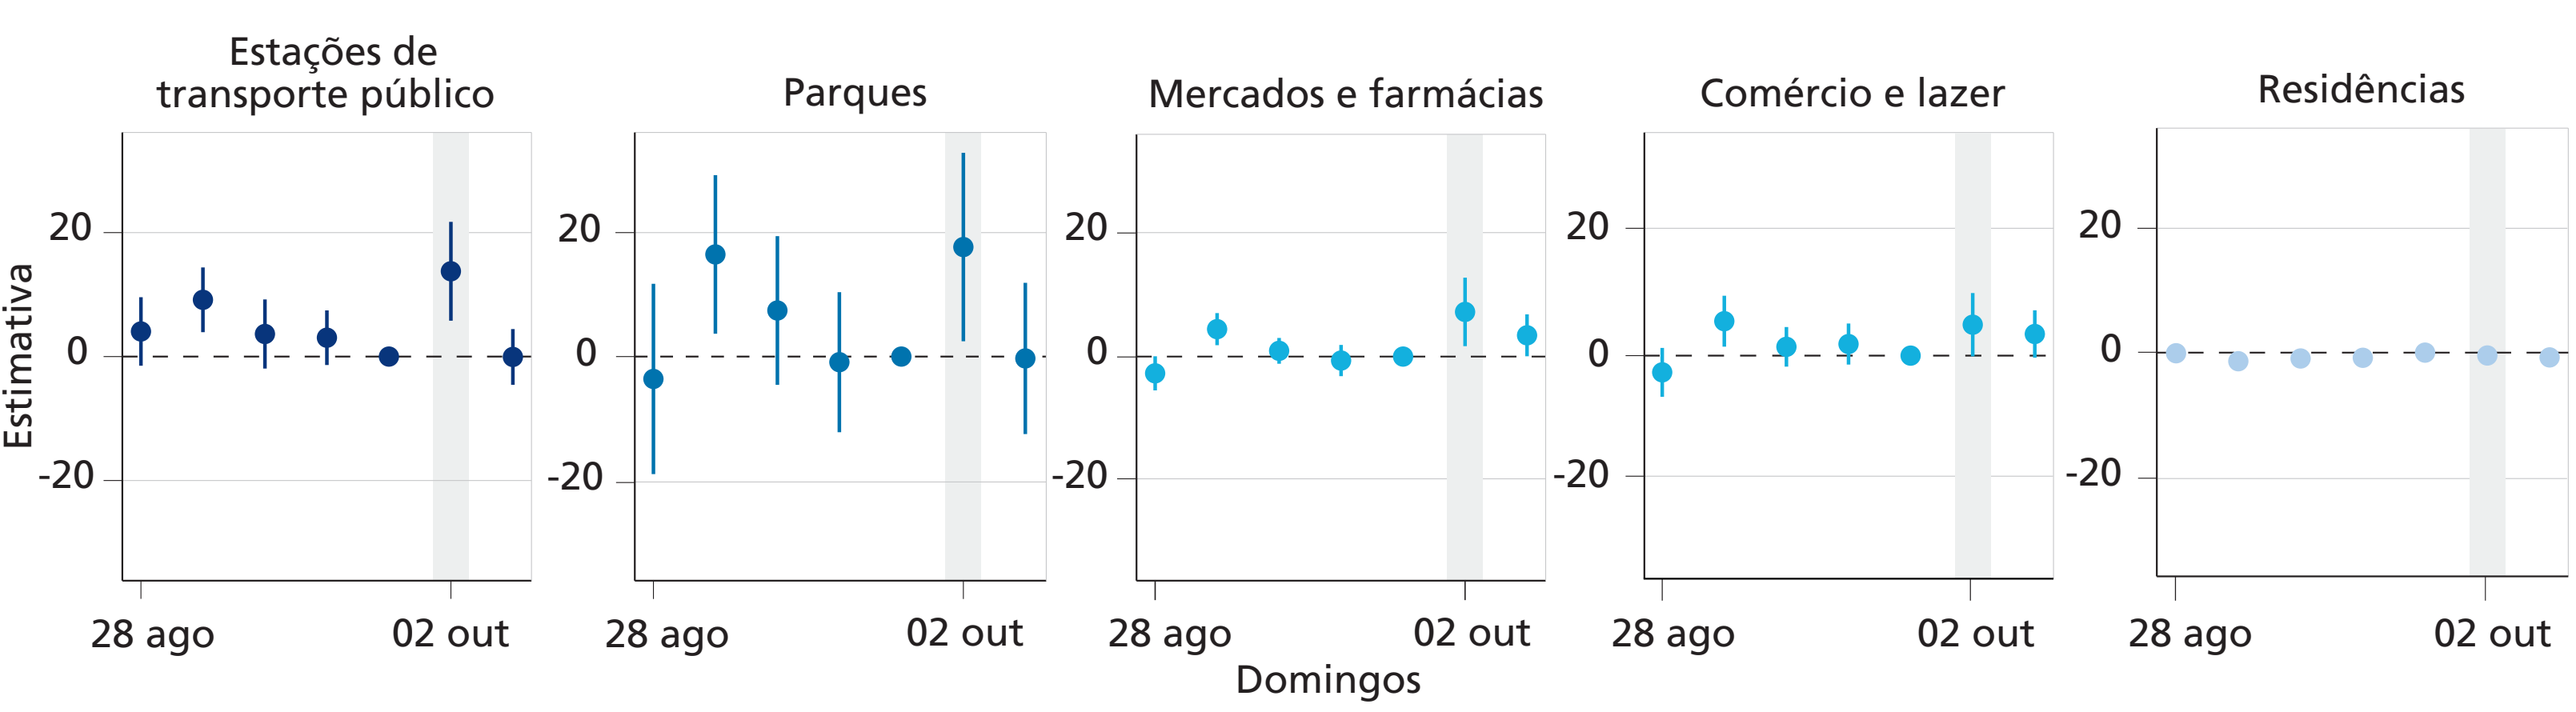
\includegraphics[width = \linewidth]{relatorios/passe-livre/graficos/pereira_mob.png}
    \subcaption*{Fonte: \cite{pereira2023transporte}}
    \label{fig_pereira_mob}
\end{figure}

Primeiramente porque no \textit{event study} apresentado (Figura \ref{fig_pereira_mob}), entre os quatro domingos anteriores, observou-se efeito significativo em um deles, mas não houve passe livre nesse domingo e os pesquisadores não comentaram nada sobre essa quebra de paralelismo no estudo. Em segundo, diferentemente do \textit{event study} para identificar efeito na abstenção, este \textit{event study} não compara o domingo de eleição com outros domingos de eleição, mas sim, com outros domingos do mês anterior. Isso é uma limitação, visto que o domingo de eleição funciona de maneira muito diferente de outros domingos e possivelmente os municípios dos grupos diferentes apresentam distintas tradições de mobilidade no dia da eleição. Nesse sentido, inclusive, que fica complicado comparar os resultados de mudança na mobilidade com mudança na abstenção, já que foram utilizados \textit{designs} diferentes no \textit{event study}.

\begin{figure}[!ht]
  \caption{Efeitos da política de passe livre no transporte público sobre: comparecimento eleitoral (A), parcela de votos para o PT (B), comparecimento em seções eleitorais com diferentes níveis socioeconômicos (C) e comparecimento em seções eleitorais em áreas com menor e maior densidade populacional (D)}
    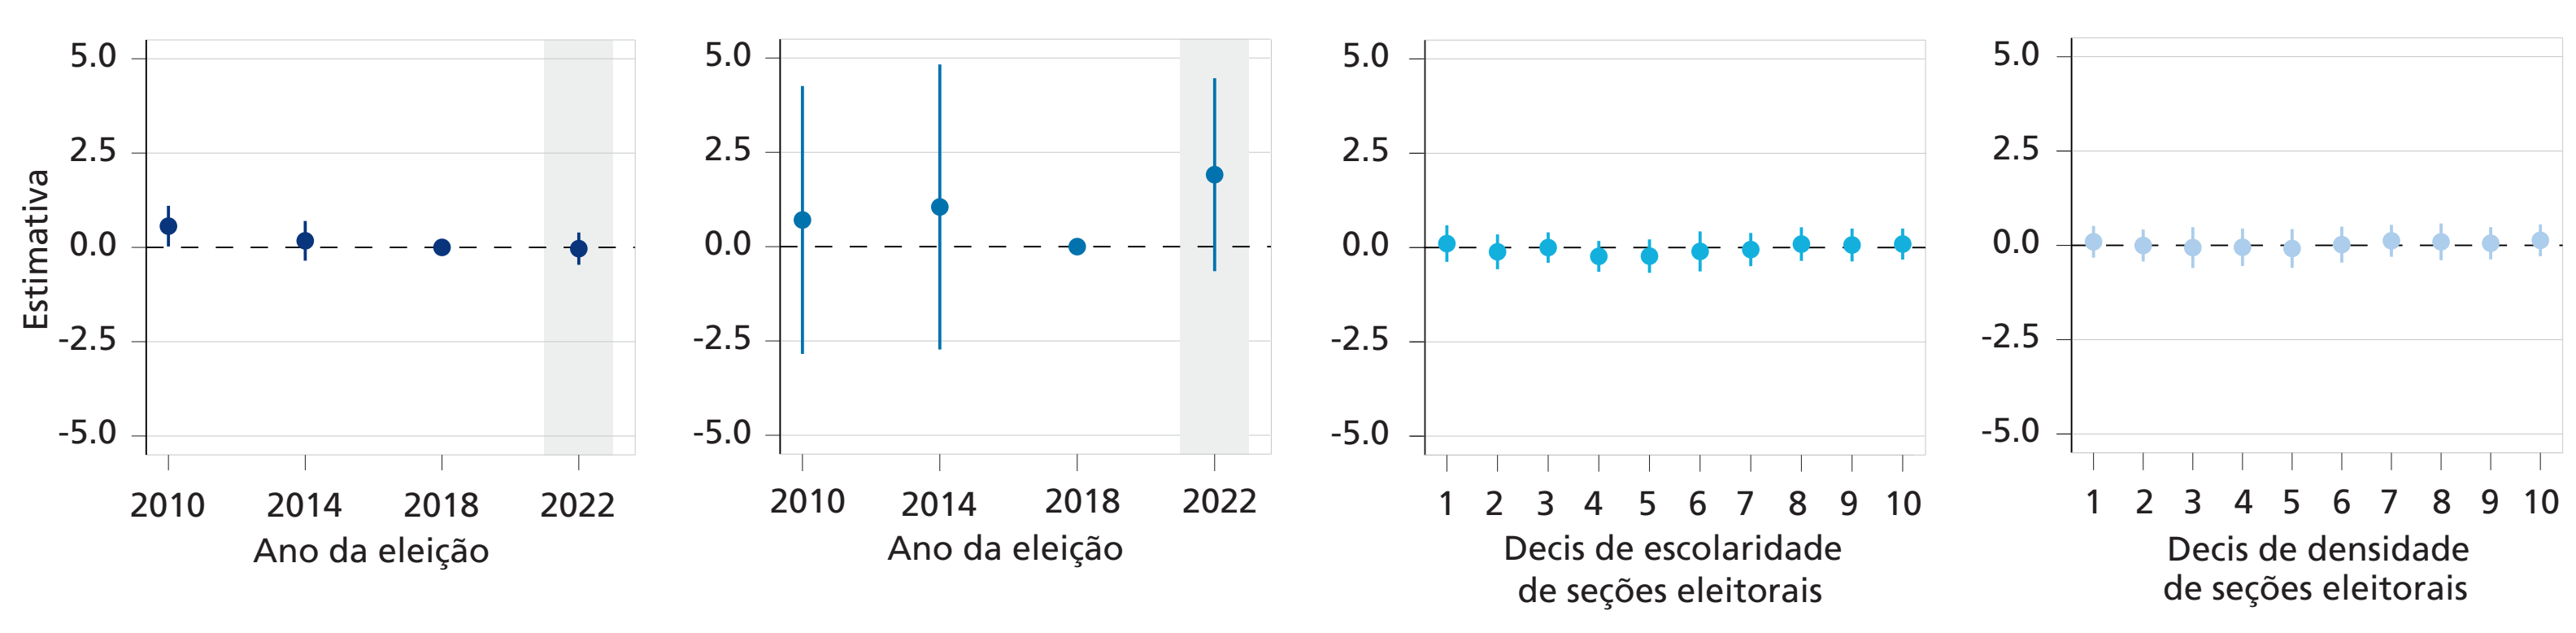
\includegraphics[width = \linewidth]{relatorios/passe-livre/graficos/pereira_abst.png}
    \subcaption*{Fonte: \cite{pereira2023transporte}}
    \label{fig_pereira_abst}
\end{figure}

Em relação a conclusão do artigo de que não houve efeito do passe livre na abstenção, novamente faltou uma discussão dos autores sobre a hipótese de identificação. No gráfico \ref{fig_pereira_abst}A, os pesquisadores medem se nos grupos de tratamento há um aumento na diferença de comparecimento do segundo e primeiro turnos em relação ao grupo de controle. Todavia, há apenas as eleições de 2010 e 2014 para fazer testes de robustez e é identificado um efeito placebo em 2010. Dessa forma, a interpretação dos resultados deveria ser que não foi possível medir o efeito do passe livre, ao invés da interpretação feita de que não houve efeito. Em outras palavras, um efeito inconclusivo é diferente de não haver efeito.

No gráfico \ref{fig_pereira_abst}C os autores fizeram uma análise de efeito heterogêneo com base em diferentes ``níveis socioeconômicos''. Entretanto, utilizaram a medida de anos de educação disponibilizada pelo TSE para separar os grupos, que é completamente defasada, visto que é apenas atualizada quando o eleitor atualiza seu título, um evento raro. Ainda sobre níveis socioeconômicos, os autores utilizam como variável de controle o PIB per capita ao longo dos anos, mas essa medida não foi divulgada para 2022 e os autores não comentaram como lidaram com essa defasagem.

De maneira geral, afirmar que o passe livre aumentou a mobilidade, mas as pessoas ao invés de votar foram aos parques implicaria ignorar todas as limitações do modelo empírico adotado na pesquisa.

\subsection{Dados}

O passe livre foi uma medida adotada em nível municipal, então os dados foram coletados também nessa escala. Para aumentar a robustez da análise, os dados foram organizados em painel, com todas as eleições nos últimos 20 anos, desde 2002. Para fins de comparação de comparáveis, foram apenas analisadas os anos de eleições presidenciais. Algumas variáveis são diferentes para o primeiro e segundo turno, como a abstenção e passe livre, mas outras como o PIB \textit{per capita} não. Os dados foram coletados para todos os municípios brasileiros.


\begin{table}
\centering
\begin{tabular}[t]{llrrrrrr}
\toprule
\multicolumn{2}{c}{ } & \multicolumn{3}{c}{Primeiro Turno} & \multicolumn{3}{c}{Segundo Turno} \\
\cmidrule(l{3pt}r{3pt}){3-5} \cmidrule(l{3pt}r{3pt}){6-8}
  & Passe Livre & Mean & SD & N & Mean & SD & N\\
\midrule
Abstenção & Não Houve & \num{0.21} & \num{0.05} & 5437 & \num{0.21} & \num{0.05} & 5148\\
 & Houve & \num{0.20} & \num{0.03} & 81 & \num{0.20} & \num{0.03} & 370\\
\bottomrule
\end{tabular}
\caption{Abstenção e tamanho amostral para cada grupo em 2022}
\label{tab_descritiva}
\end{table}

\textcite{smets2013embarrassment} conduziram uma meta análise de 90 estudos empíricos que foram publicados nos jornais de maior renome durante a década de 2000 que estudaram a abstenção de votos. Como variáveis a nível individual que foram consideradas relevantes, estão a idade, escolaridade e renda. Os dados do TSE são segmentados por faixa etária, gênero e escolaridade, mas o dado da escolaridade não é de qualidade, visto que não é atualizado regularmente - apenas quando há uma atualização do título de eleitor. Para contornar este problema, seria ideal analisar pela PNAD a média de anos de estudo na população, mas dessa forma não haveria cobertura de todos os municípios do Brasil. A \textit{proxy} adotada foi a nota do IDEB do município, um índice de educação básica calculado com base no Censo Escolar e desempenho no Sistema de Avaliação da Educação Básica (Saeb). Quanto aos dados de renda, os dados de PIB \textit{per capita} a nível municipal foram coletados do IBGE.

Para fazer o balanceamento dos grupos, foram utilizadas algumas variáveis do censo de 2010. Apesar do censo estar bastante desatualizado, as variáveis se referem a fatores estruturais dos municípios, que não mudam muito ao longo do tempo, então o viés não é muito significativo.

Em relação às variáveis do modelo microeconômico, nem todos os componentes são observáveis. O $\alpha$ e $B_s$, por exemplo, são extremamente subjetivos, o que os torna praticamente imensuráveis. A literatura identificou alguns fatores que podem contribuir com o dever cívico do voto, $D$, como a participação da população em organizações políticas, filiação partidária, número de funcionários públicos, etc. A maioria desses fatores são invariantes no tempo e são relacionados à cultura do município. Uma variável de controle adotada foi a participação do governo no PIB municipal, também obtida através do IBGE. 

Em relação ao custo de votar, muitos componentes estão envolvidos. Entre eles, o custo do transporte, a distância às urnas, demora e filas, chuvas fortes, etc. Pela dificuldade de mensurar esses fatores, foi adotada apenas uma variável mensurável, que é o número de eleitores por urna - pode indicar se há grandes filas. Foram coletados os dados históricos pluviométricos disponibilizados pelo INMET para identificar se choveu no dia da eleição, mas há muitos dados faltantes, o que pode prejudicar a análise, inviabilizando a utilização desses dados. Já os componentes $K, E, N, t$ são obtidos ou calculados através dos dados do TSE e IBGE.

A descrição mais detalhada das variáveis adotadas se encontra na tabela \ref{tab_variaveis}.

\begin{table}
    \centering
    \caption{Variáveis utilizadas nos modelos econométricos}

    \begin{tabular}{m{0.18\linewidth}|m{0.7\linewidth}}
        Variável & Descrição \\
        \toprule
        Tratamento & Variável binária que assume 1 caso o município tenha recebido passe livre e 0 caso contrário \\
        \midrule
        Competitividade & Quão proximos foram os resultados entre primeiro e segundo candidatos. Calculado por $1/[\log({V_A/V_B})]$, na qual $V_A$ representa o número de votos recebidos pelo candidato mais votado e $V_B$, pelo segundo candidato mais votado.\footnotemark \\
        \midrule
        População & População do município \\
        \midrule
        PIB per capita & PIB per capita do municipio, disponível até 2020. Para 2022, foram utilizados os últimos dados disponíveis, de 2020. \\
        \midrule
        Beneficiados & Número de pessoas no municipio dividido pela quantidade de eleitores aptos. \\
        \midrule
        IDEB & Nota da educacao dos anos finais do ensino fundamental nas escolas publicas. A nota é apenas calculadas nos anos ímpares, com o primeiro dado disponível em 2005, então foram utilizados dados defasados em um ano. \\
        \midrule
        PIB governo & É definido como valor adicionado bruto a preços correntes da administração, defesa, educação e saúde públicas e seguridade social dividido pelo PIB municipal. \\
        \midrule
        Eleitores por seção & Média do número de eleitores aptos por seção eleitoral no município

    \end{tabular}

    \label{tab_variaveis}
\end{table}

\footnotetext[\thefootnote]{competitividade calculada pós}

% \begin{table}
%     \centering
%     \begin{tabular}[t]{llrrrrrr}
%     \toprule
%     \multicolumn{2}{c}{ } & \multicolumn{3}{c}{Primeiro Turno} & \multicolumn{3}{c}{Segundo Turno} \\
%     \cmidrule(l{3pt}r{3pt}){3-5} \cmidrule(l{3pt}r{3pt}){6-8}
%       & Passe Livre & Mean & SD & N & Mean & SD & N\\
%     \midrule
%     Abstenção & Não Houve & \num{0.21} & \num{0.05} & 5437 & \num{0.21} & \num{0.05} & 5148\\
%      & Houve & \num{0.20} & \num{0.03} & 81 & \num{0.20} & \num{0.03} & 370\\
%     \bottomrule
%     \end{tabular}
%     \caption{Abstenção e tamanho amostral para cada grupo em 2022}
%     \label{tab_descritiva}
%     \end{table}

\subsection{Metodologia}

A estratégia adotada foi de realizar um \textit{diff-in-diff} com efeitos fixos de tempo e município no qual o grupo de tratamento é composto pelos municípios que adotaram o passe livre e o de controle, pelos que não adotaram. A hipótese de identificação é de que os grupos apresentam trajetórias de abstenção paralelas ao longo das eleições e, portanto, caso a diferença entre os grupos mude apenas no ano de tratamento, isso é consequência do tratamento.

\begin{equation}
\label{eq_econometric}
    \log{(y_{it})}=\beta\text{Passe Livre}_{it} + X_{it}\gamma + \alpha_t + \delta_i + \epsilon_{it}
\end{equation}

Na equação \ref{eq_econometric}, $y_{ti}$ representa a abstenção no ano $t$ para o município $i$ e $X_{it}$ representa um vetor de covariantes. O coeficiente $\beta$ captura o efeito médio do passe livre no $\log$ da abstenção e $\alpha_t$ e $\delta_i$ representam os efeitos fixos de tempo e município, respectivamente. A variável Passe Livre assume o valor 1 em 2022 para os municípios que adotaram o passe livre, caso contrário, assume zero. As estimações foram feitas separadamente para o primeiro e segundo turnos. 

A variável passe livre é endógena, já que não foi decidido de forma aleatória qual município adotaria o passe livre. Portanto, a hipótese de identificação não se sustenta, pois os grupos de controle e tratamento são muito diferentes e não podem ser comparados diretamente. Para lidar com essa questão, foi utilizado o método do \textit{Propensity Score Matching}, no qual calcula-se a probabilidade do passe livre ser adotado e compara-se municípios com propensões a ser tratados parecidas. O PSM foi calculado a partir do \textit{Nearest Neighbor} ou ``vizinho mais próximo'' com reposição.

Como discutido e observado na Figura \ref{fig_staticA}, mudanças no custo afetam de forma diferente municípios que apresentam diferentes faixas de abstenção. Nesse sentido, a modelagem da abstenção em termos logarítmicos lineariza essa relação, diminuindo o viés oriundo da heterogeneidade. 

\subsection{Resultados empíricos}

Considerando a endogeneidade discutida, o primeiro passo adotado foi fazer o \textit{Propensity Score Matchin}g (PSM). Na figura \ref{fig_balanceamento} é possível observar o suporte comum antes e depois de aplicar o método do PSM. O eixo $x$ dos gráficos se refere à probabilidade do município receber o tratamento, enquanto o $y$ se trata da densidade de probabilidade. Na figura \ref{fig_posPSM} identifica-se uma grande sobreposição nas probabilidades dos grupos de receber o tratamento, uma evidência de que os municípios que estão sendo comparados são muito semelhantes, menos em relação a receber o tratamento. O suporte comum é menos significativo no primeiro turno porque menos municípios foram tratados, então é mais difícil de encontrar vizinhos próximos.

\begin{figure}[!ht]
  \caption{Balanceamento dos grupos antes e depois do \textit{Propensity Score Matching} (PSM)}
    \begin{subfigure}[t]{0.49\linewidth}
      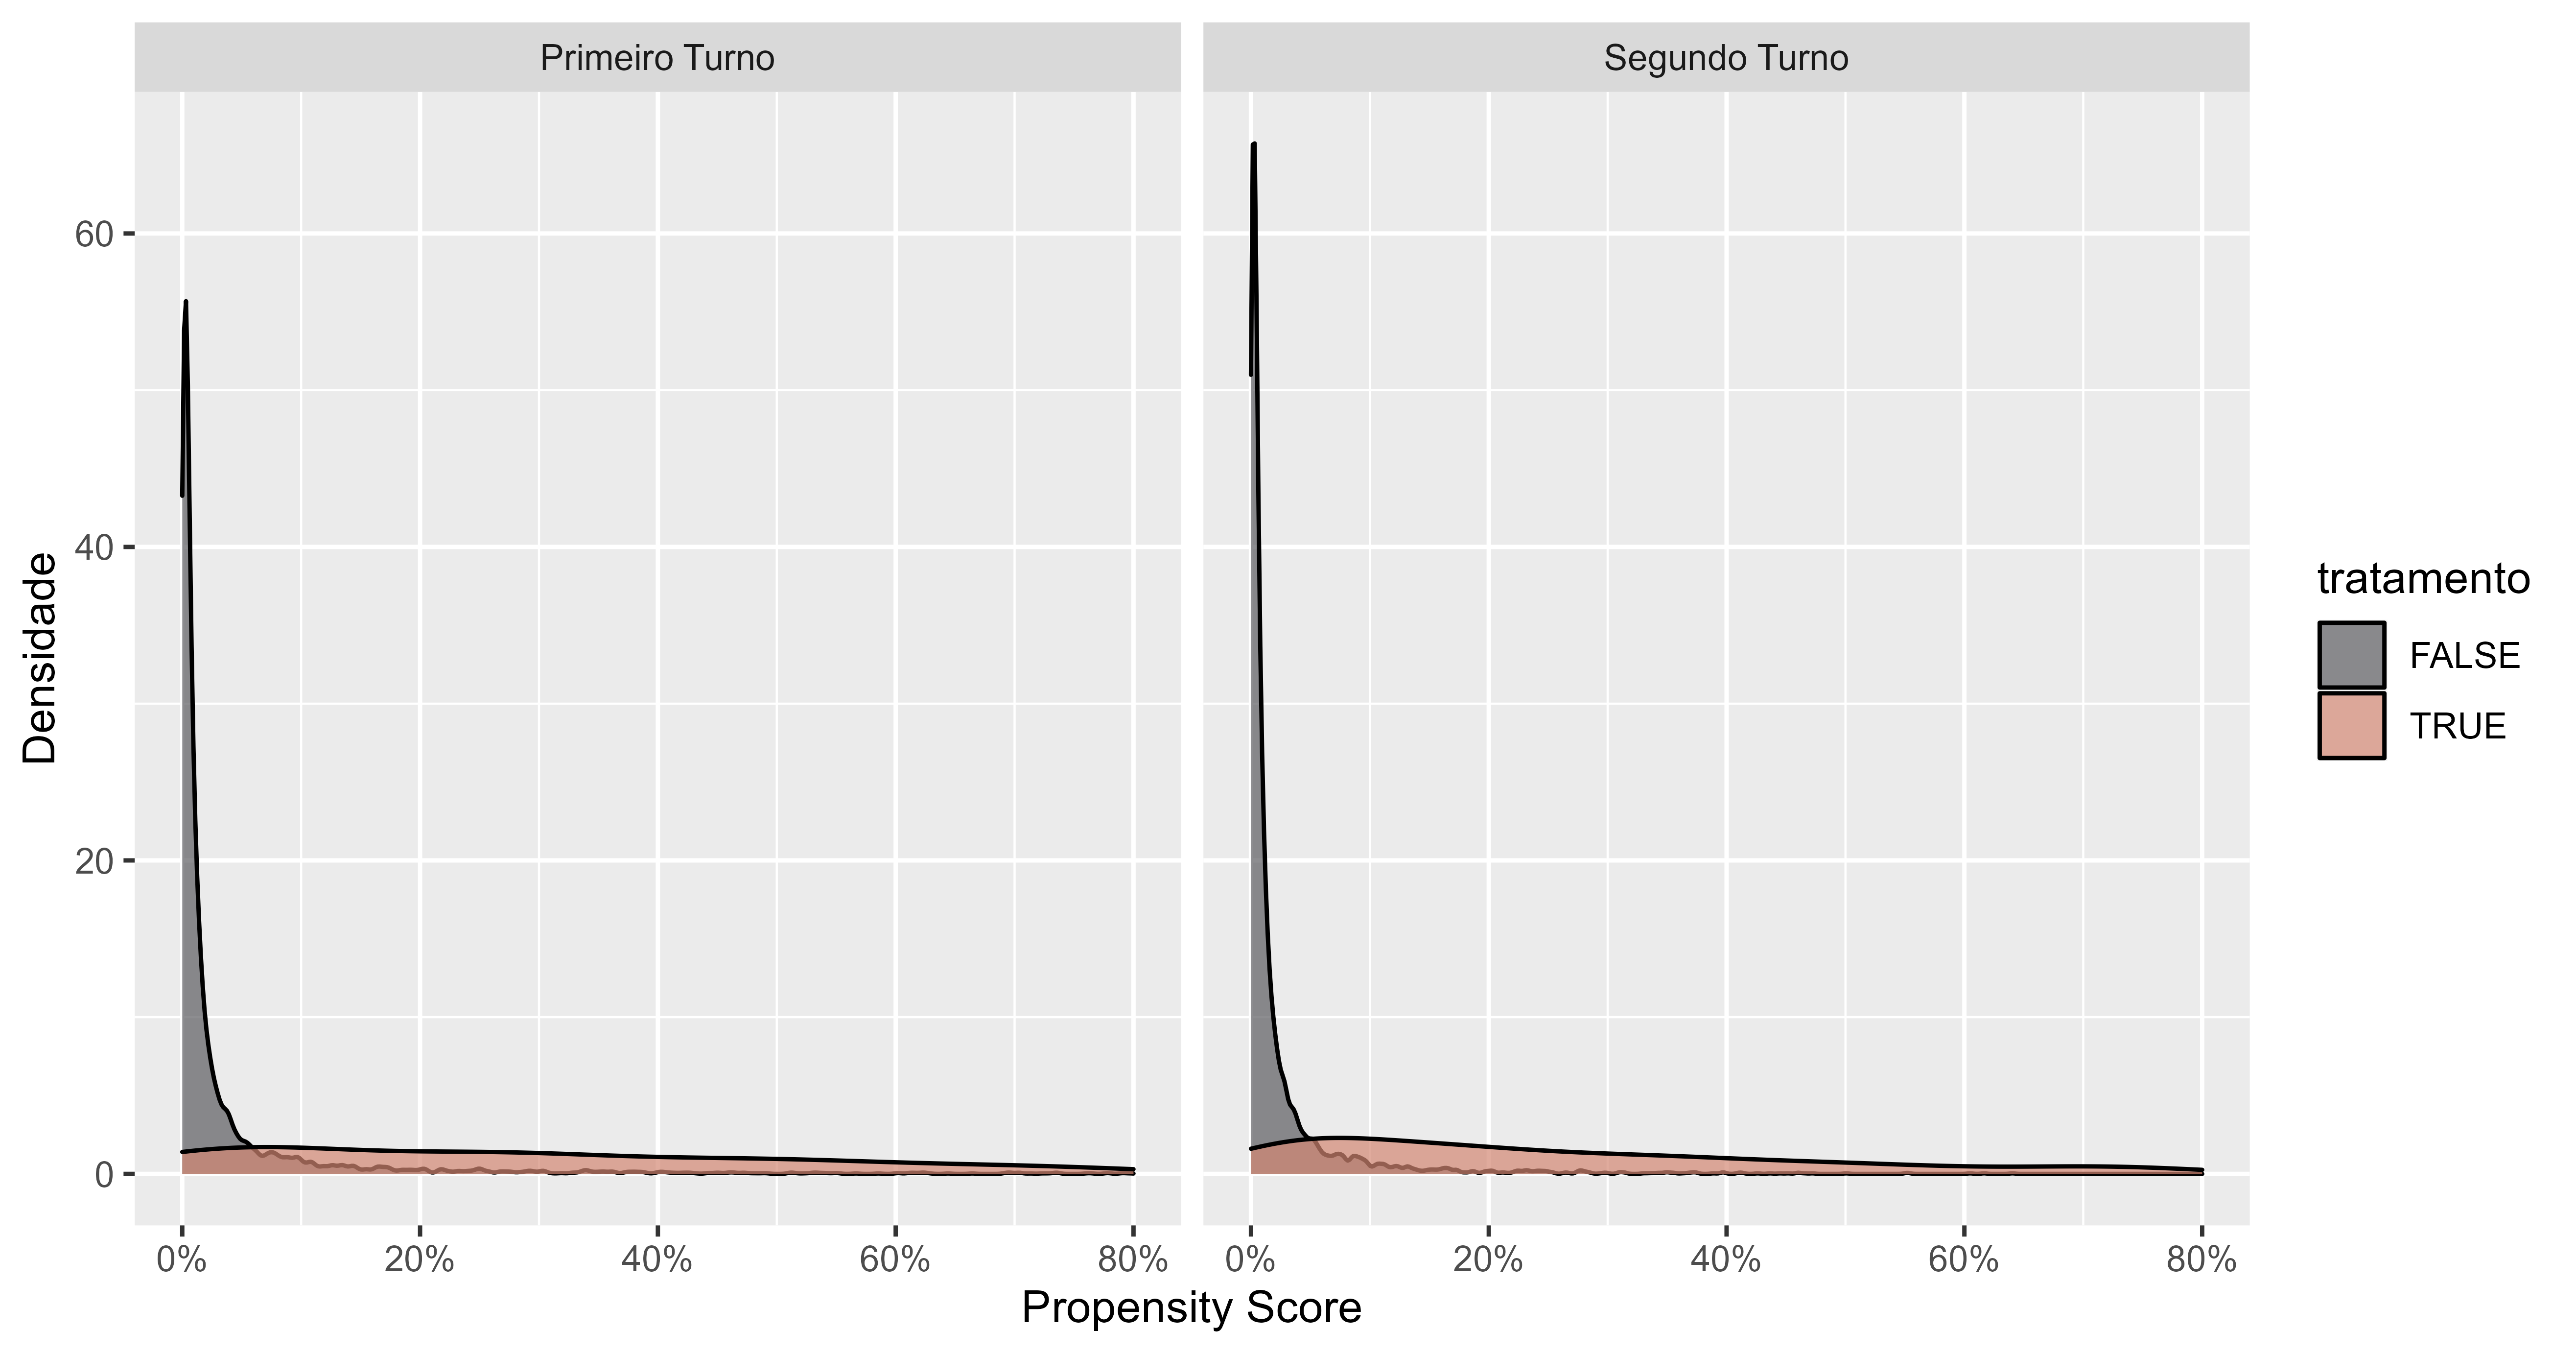
\includegraphics[width = \linewidth]{relatorios/passe-livre/graficos/pre-propensity.png}
      \caption{Antes do PSM}
      \label{fig_prePSM}
    \end{subfigure}
    \hfill
    \begin{subfigure}[t]{0.49\linewidth}
      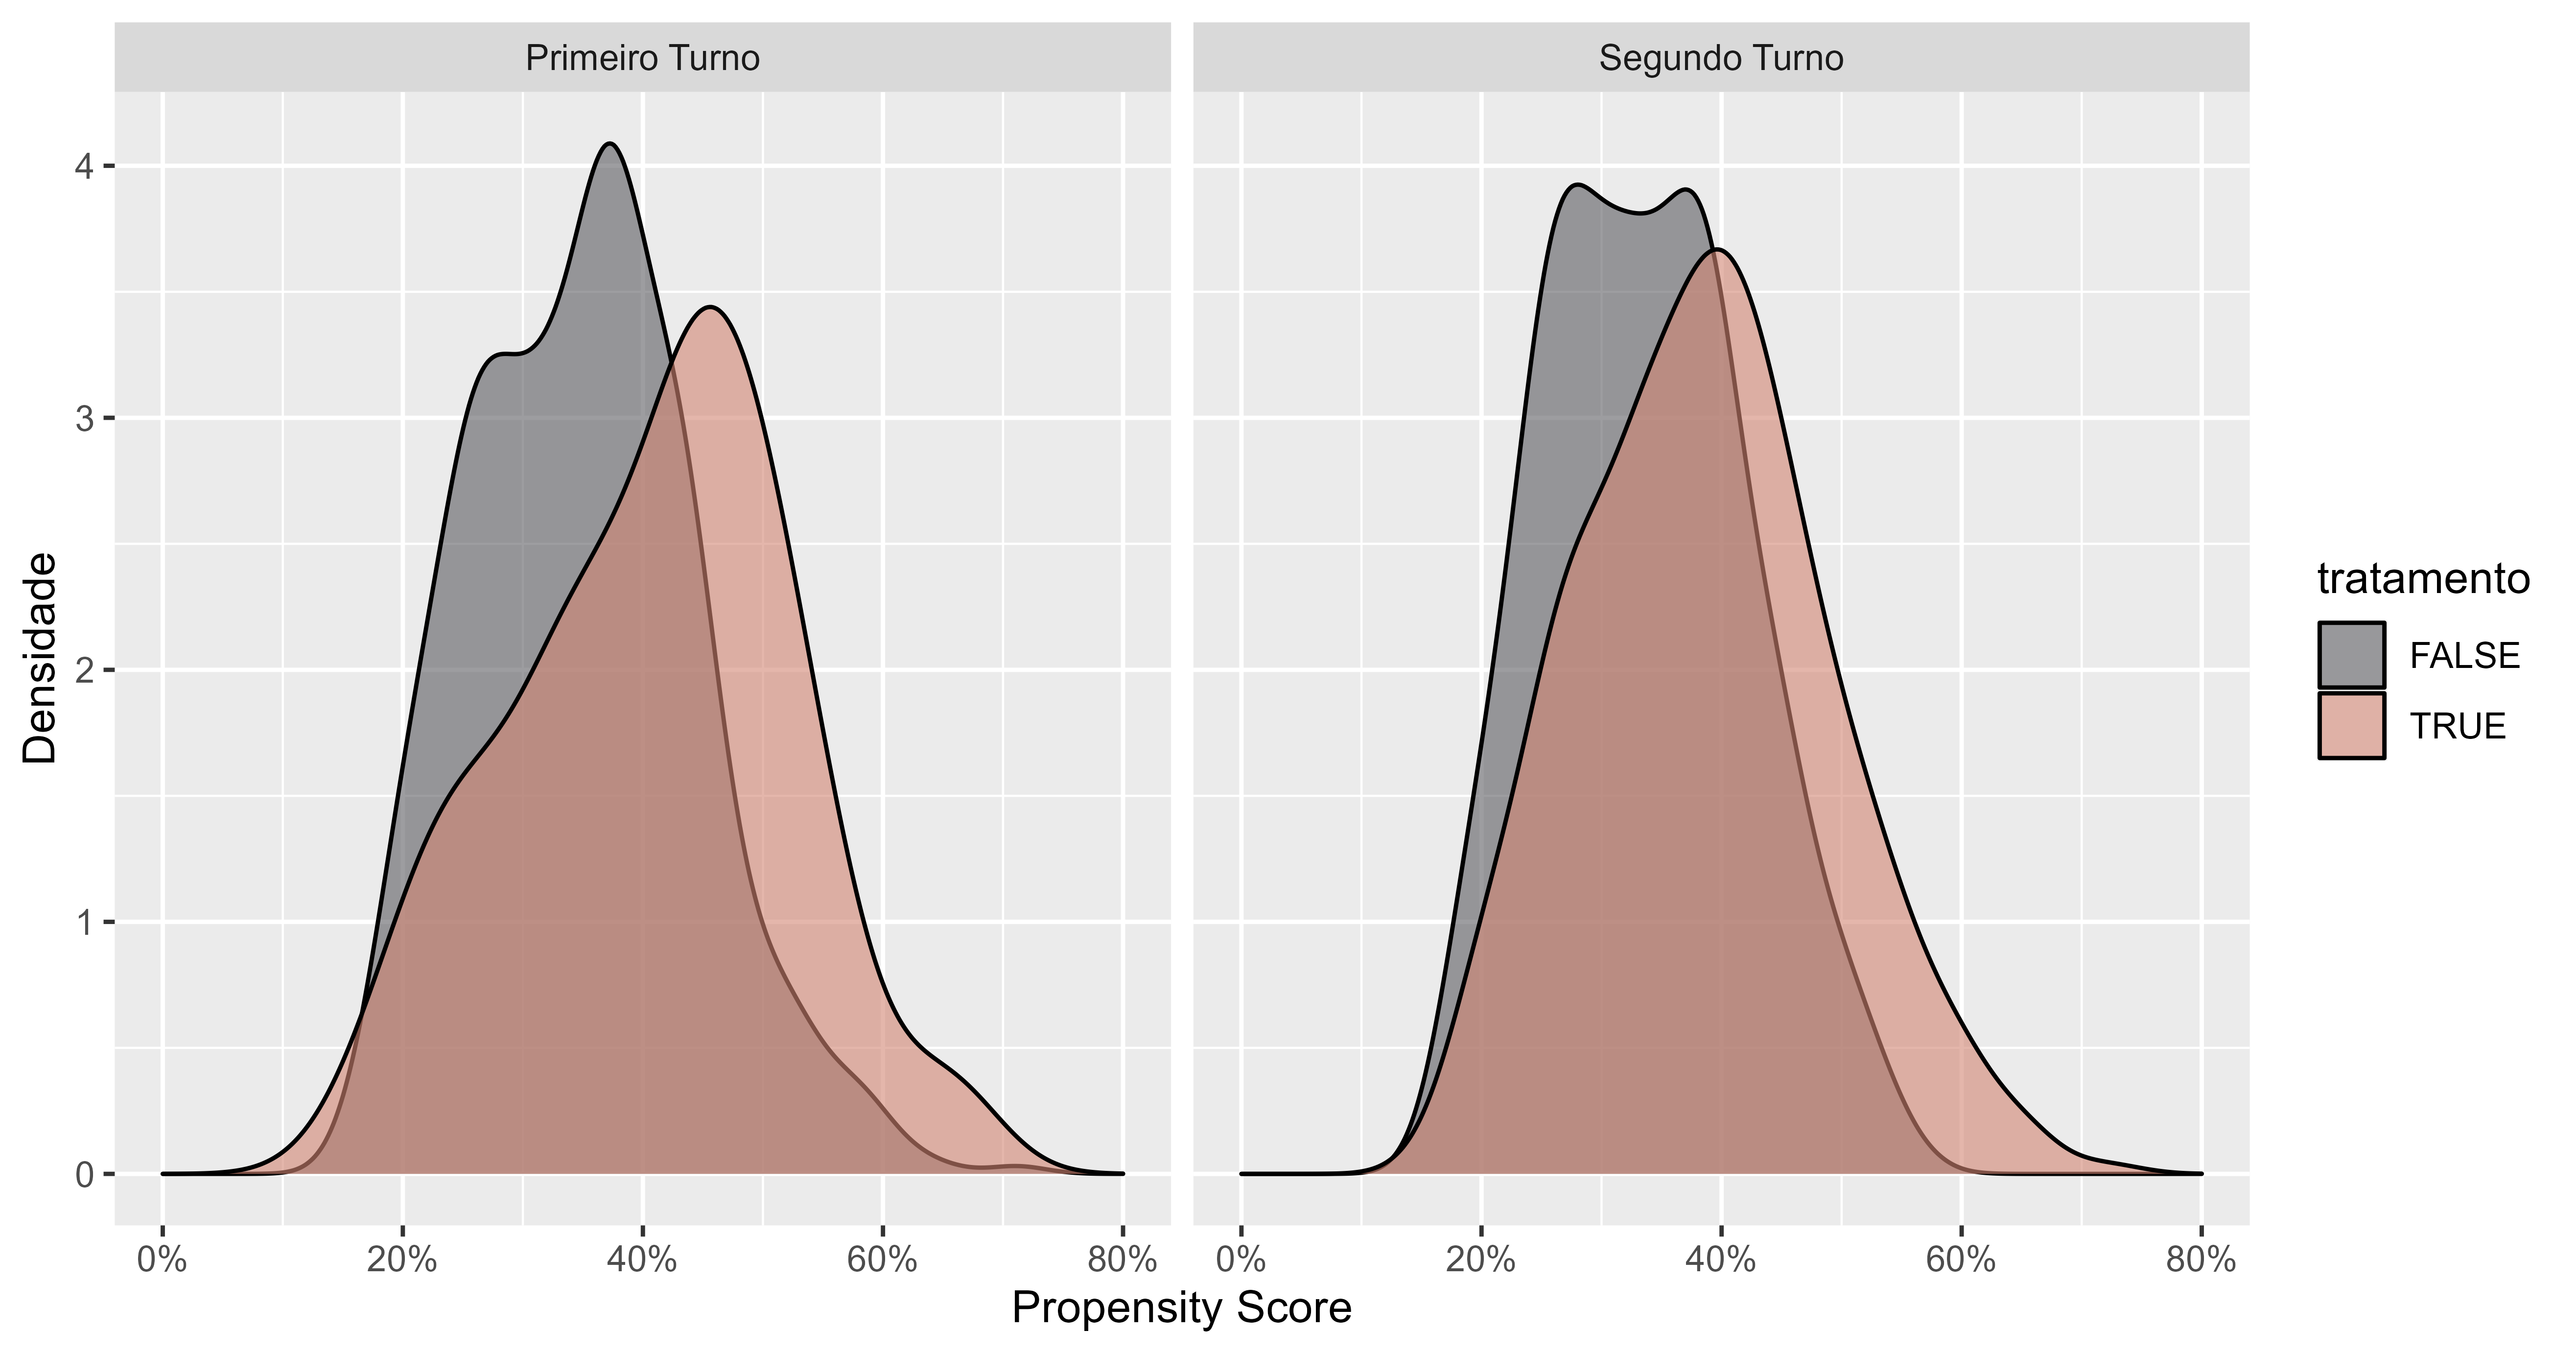
\includegraphics[width = \linewidth]{relatorios/passe-livre/graficos/pos-propensity.png}
      \caption{Depois do PSM}
      \label{fig_posPSM}
    \end{subfigure}
    \label{fig_balanceamento}
  \end{figure}

Depois do balanceamento dos grupos, foi conduzido um \textit{event study} (Tabela \ref{tab_eventStud}), para que se verifique a paralelidade das tendências dos diferentes grupos a partir de testes placebos. Foi escolhido como referência o ano de $t-1$, que neste caso é 2018. Caso se identifique efeito no tratamento em um ano que não teve tratamento, há uma forte evidência de que as trajetórias não são paralelas. O \textit{event study} foi conduzido com variáveis controle e sem. A descrição detalhada das variáveis se encontra na tabela \ref{tab_variaveis}.

A partir dos resultados da tabela \ref{tab_eventStud}, a hipótese de identificação não se sustenta para o primeiro turno, visto que foi observado um efeito do passe livre na abstenção em 2014, para o nível de significância de 5\%, o que é impossível, visto que não houve passe livre em 2014. Para o segundo turno não há evidências que rejeitem a hipótese de paralelismo das tendências, mas também não há evidências que apontem para um efeito do passe livre na abstenção.

\begin{table}
\centering
\begin{tabular}[t]{lcccc}
\toprule
& \multicolumn{2}{c}{Sem Controles} & \multicolumn{2}{c}{Com Controles} \\
  \cmidrule(lr){2-3} \cmidrule(lr){4-5}
  & Primeiro Turno & Segundo Turno & Primeiro Turno & Segundo Turno\\
\midrule
tratamento:2002 & \num{-0.069} (\num{0.290}) & \num{0.044} (\num{0.216}) &  & \\
tratamento:2006 & \num{-0.044} (\num{0.379}) & \num{0.024} (\num{0.451}) & \num{-0.049} (\num{0.273}) & \num{0.027} (\num{0.238})\\
tratamento:2010 & \num{-0.068} (\num{0.196}) & \num{0.003} (\num{0.904}) & \num{-0.069} (\num{0.109}) & \num{0.008} (\num{0.681})\\
tratamento:2014 & \num{-0.146} (\num{0.005}) * & \num{-0.010} (\num{0.627}) & \num{-0.090} (\num{0.023}) * & \num{-0.001} (\num{0.956})\\
tratamento:2022 & \num{-0.010} (\num{0.692}) & \num{0.016} (\num{0.182}) & \num{-0.026} (\num{0.282}) & \num{0.003} (\num{0.803})\\
log(Competitividade) &  &  & \num{-0.024} (\num{<0.001}) * & \num{-0.010} (\num{0.018}) *\\
log(PIB per capita) &  &  & \num{-0.022} (\num{0.043}) * & \num{-0.016} (\num{<0.001}) *\\
log(Beneficiados) &  &  & \num{-0.865} (\num{<0.001}) * & \num{-0.857} (\num{<0.001}) *\\
IDEB &  &  & \num{-0.063} (\num{0.002}) * & \num{-0.062} (\num{<0.001}) *\\
log(População) &  &  & \num{0.176} (\num{0.287}) & \num{0.164} (\num{0.089})\\
log(PIB governo) &  &  & \num{-0.018} (\num{0.005}) * & \num{-0.011} (\num{<0.001}) *\\
log(Eleitores por seção) &  &  & \num{0.711} (\num{<0.001}) * & \num{0.298} (\num{<0.001}) *\\
\midrule
Num.Obs. & \num{972} & \num{4440} & \num{802} & \num{3656}\\
R2 & \num{0.567} & \num{0.590} & \num{0.706} & \num{0.709}\\
R2 Adj. & \num{0.483} & \num{0.526} & \num{0.631} & \num{0.651}\\
R2 Within & \num{0.021} & \num{0.004} & \num{0.276} & \num{0.184}\\
R2 Within Adj. & \num{0.015} & \num{0.002} & \num{0.263} & \num{0.181}\\
\bottomrule
\end{tabular}
\caption{Resultado do \textit{event study} com efeito fixo de tempo e município, estimações por MQO}
\label{tab_eventStud}
\end{table}

É relevante destacar que as variáveis de controle selecionadas se mostraram bastante relevantes e apresentam o sinal esperado, o que aponta na mesma direção da literatura teórica e outros estudos empíricos. Os coeficientes do primeiro turno são semelhantes aos do segundo turno, com exceção da competitividade e eleitores por seção, que se mostram menos relevantes no segundo turno. Entretanto, a variável de interesse a partir dessa estratégia não se demonstra relevante.

Com isso, foi feita uma análise de efeito heterogêneo de renda. Como descrito com melhor detalhe na seção \ref{subsec_revisLit} e na figura \ref{fig_static2}, uma redução no custo de votar afeta de formas diferentes cada município e uma variável importante que define essa diferença é o nível de renda do município. Portanto, foram separados os municípios em 4 quantis de renda e foi conduzido novamente o \textit{event study} separadamente para cada um desses grupos (Figura \ref{fig_eventStud}). 

\begin{figure}[!ht]
  \caption{Análise de efeito heterogêneo através de um \textit{event study}}
    \begin{subfigure}[t]{0.49\linewidth}
      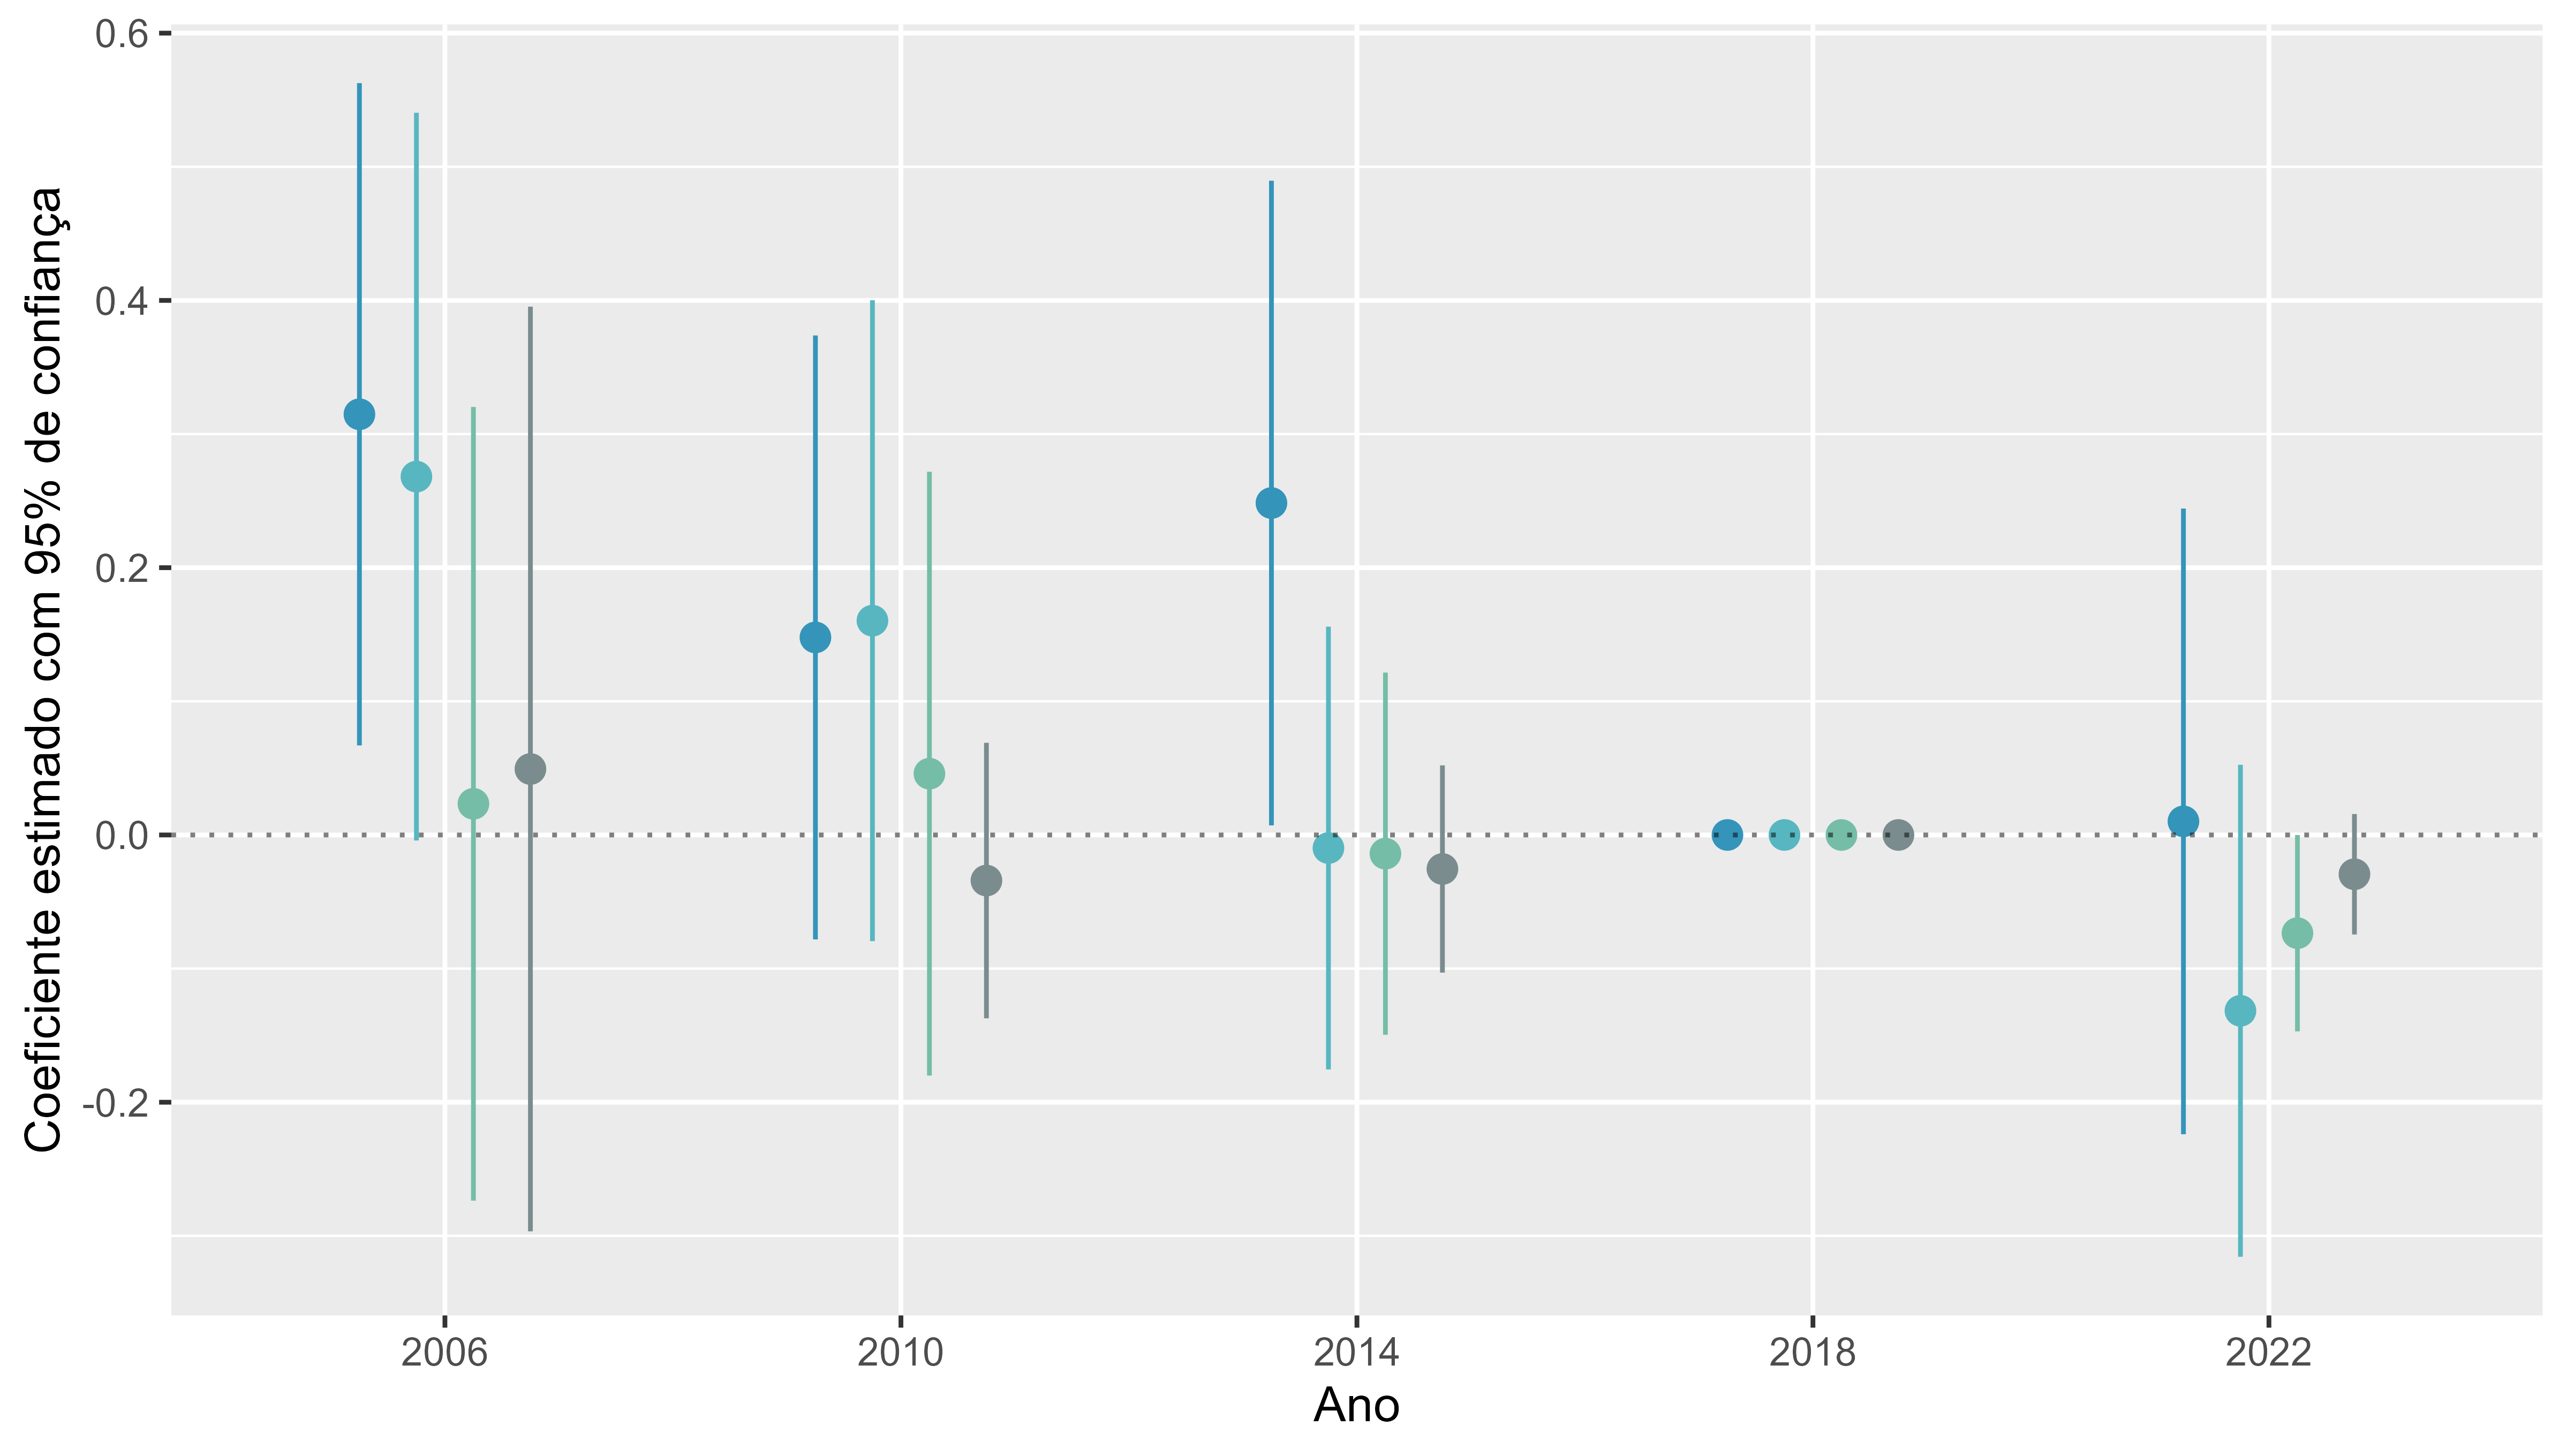
\includegraphics[width = \linewidth]{relatorios/passe-livre/graficos/event_study_heter_1t.png}
      \caption{Primeiro Turno}
      \label{fig_eventStud1}
    \end{subfigure}
    \hfill
    \begin{subfigure}[t]{0.49\linewidth}
      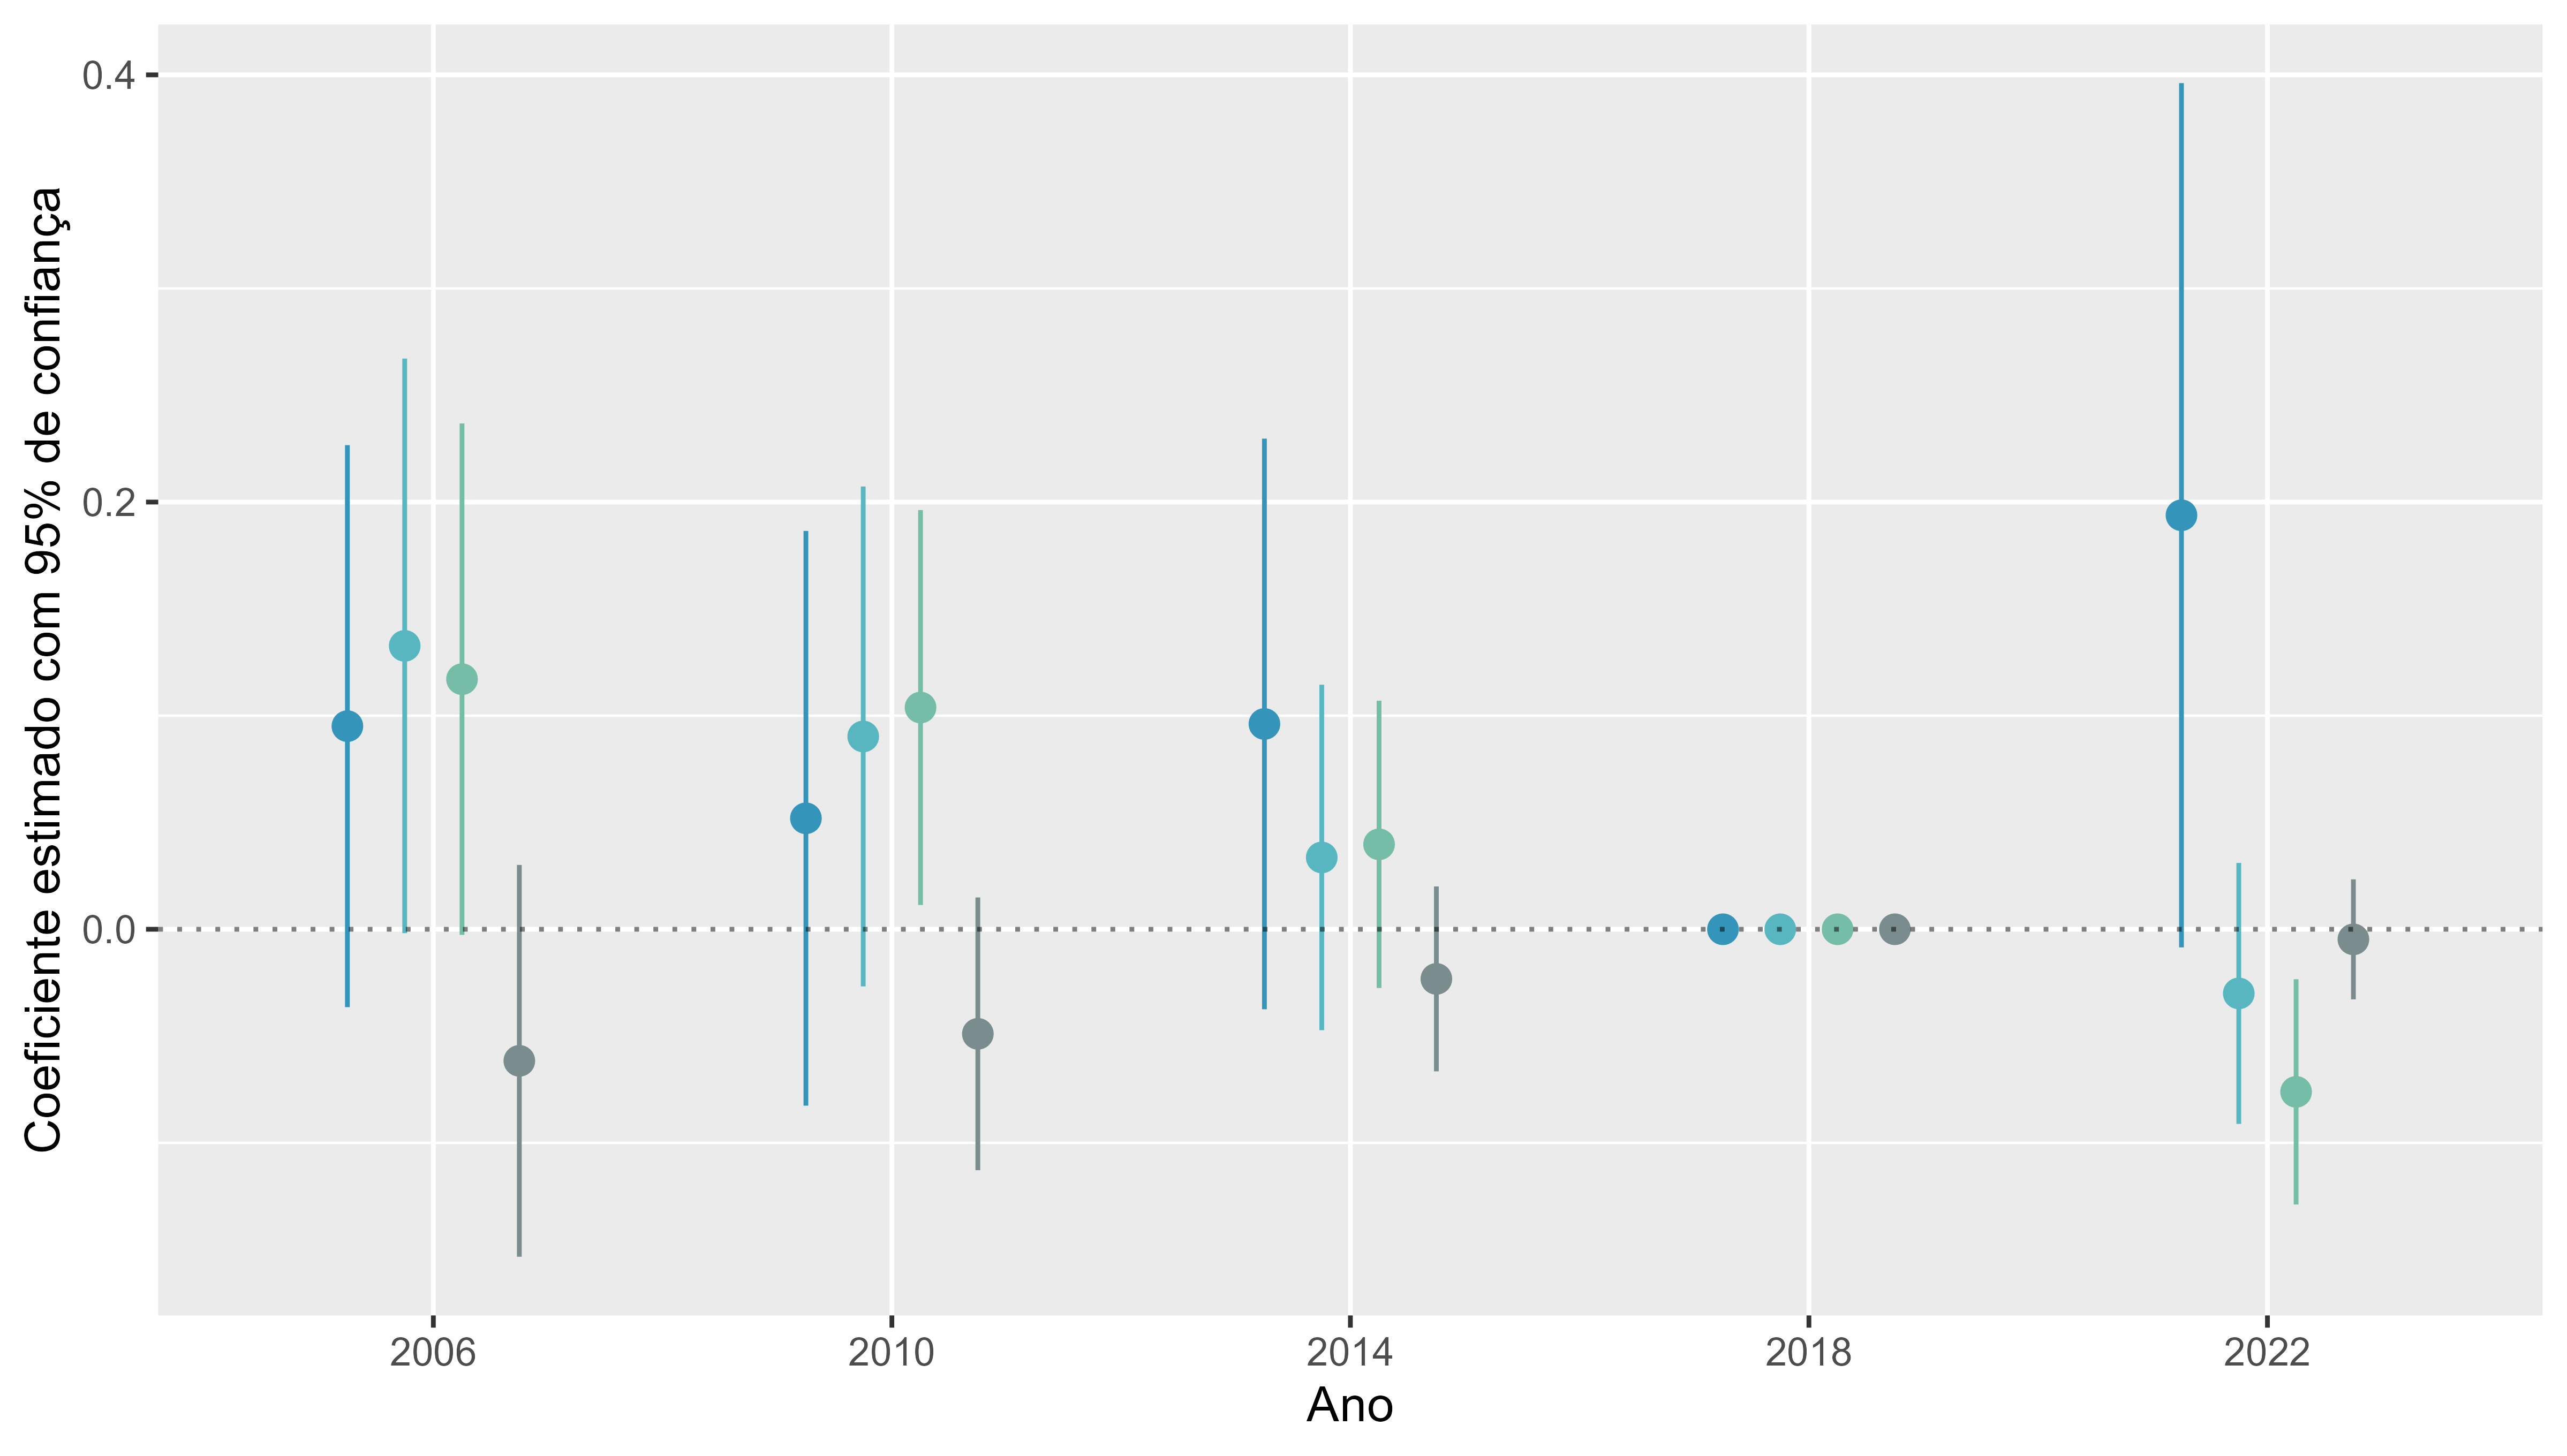
\includegraphics[width = \linewidth]{relatorios/passe-livre/graficos/event_study_heter_2t.png}
      \caption{Segundo Turno}
      \label{fig_eventStud2}
    \end{subfigure}
    
    \subcaption*{O quartil à esquerda se refere ao quartil mais pobre e o da direita, o mais rico}

    \label{fig_eventStud}
  \end{figure}

A partir da análise da Figura \ref{fig_eventStud}, fica evidente a dificuldade de validar a hipótese de identificação, visto que com 95\% de confiança observa-se mais de uma vez efeito placebo em anos de eleição nas quais não houve tratamento, principalmente quando a amostra é dividida em quatro e perdem-se muitos graus de liberdade. Entretanto, para o terceiro quartil de renda foi identificada uma redução na abstenção do segundo turno com 5\% de significância. Com base nos resultados do \textit{event study} como um todo, o efeito do passe livre na abstenção é inconclusivo utilizando a estratégia empírica escolhida, dada a fragilidade da hipótese de identificação.

\subsection{Limitações}

A principal limitação do estudo empírico conduzido, como mencionado anteriormente, foi a dificuldade de validar a hipótese de identificação da metodologia escolhida. Como o intervalo de tempo de quatro anos entre as eleições é muito grande, muitos fatores em um município mudam de uma votação para outra e depois de apenas 5 eleições, já se passaram 20 anos, tornando eleições distantes praticamente incomparáveis do ponto de vista empírico. Nesse sentido, seria importante conduzir um estudo com um método que não precise comparar os resultados de 2022 com a eleição anterior.

Outra dificuldade é oriunda da endogeneidade na decisão de adotar ou não o tratamento. Mesmo depois do balanceamento dos grupos, eles se mostraram não tão comparáveis, o que indica que o perfil de município que adotou o passe livre é bastante diferente do perfil dos que não adotaram. Informações como se o município escolheu adotar o passe livre ou foi obrigado a fazê-lo podem ajudar a entender o perfil do município tratado e balancear melhor os grupos.

Além disso, há uma grande defasagem nas variáveis. O PIB \textit{per capita}, por exemplo não foi divulgado ainda para o ano de 2022, e foi necessário utilizar o dado desatualizado de 2020, o que pode gerar viés. Ademais, as variáveis utilizadas para o balanceamento, estão defasadas em 12 anos. Como já foi discutido, essa defasagem não é tão importante quanto a dos dados para a regressão principal, mas ainda merece ser destacada.

A cobertura do sistema de transporte público do município determina quantas pessoas efetivamente conseguem usufruir do benefício do passe livre e para resultados mais robustos isso teria que ser considerado. Por fim, como discutido na seção teórica, a assimetria de informação é uma variável extremamente relevante para determinar o sucesso ou fracasso do passe livre e isso não foi contabilizado ou considerado na análise empírica. 

\section{Conclusão}

Pelas limitações e dificuldades apresentadas, os resultados empíricos em relação ao efeito do passe livre na abstenção são inconclusivos. Nesse sentido, o único resultado que pode ser validado é o teórico. O que a teoria microeconômica indica é que, assumindo as premissas do modelo, uma redução no custo do voto leva a um maior comparecimento quando não há assimetria de informação, mesmo que muito pequeno. Entretanto, não há evidências de que o passe livre foi adotado de maneira eficiente \footnote{Eficiente se refere à uma maneira que todos os habitantes estão cientes da medida e que ela não gere assimetria de informação. Neste caso, os eleitores antecipariam de maneira correta a quantidade de pessoas que seriam ``convencidas'' a votar, mesmo que seja apenas 1 pessoa}, então pode ser que a medida realmente não tenha apresentado efeito de reduzir a abstenção em 2022.

Por outro lado, o que a teoria indica é que se um município adotar o passe livre de maneira eficiente, a abstenção será reduzida. Na medida em que a adoção é mais ineficiente, têm-se um \textit{moral hazard} e, como discutido na figura \ref{fig_static4}, o efeito do passe livre pode ser atenuado ou pode até acabar sendo o efeito contrário em um caso extremo. 

Nesse sentido, caso seja adotada a medida, há alguns pontos importantes para serem levados em conta. Primeiramente, é muito importante garantir que os canais de comunicação do governo trabalhem de forma a fazer a notícia chegar em todos, principalmente aqueles que usufruem do sistema de transporte público. Em segundo, no dia da eleição a capacidade e qualidade do transporte entregues devem ser igual ou melhor do que o prometido, para evitar que aconteça o \textit{moral hazard}.

\relatorio{Estudo e Predição da Exposição de Liquidez de Capital}
    {
        \noindent Pesquisador: Esdras Gomes Carvalho

        \noindent Orientador: Ivar Alberto Glasherster Lange Hartmann
    }
    {O presente projeto visa auxiliar o entendimento e análise do padrão de votação dos ministros do Supremo Tribunal Federal (STF) do Brasil. Dada a relevância do judiciário e a complexidade em acessar os dados dos processos, a pesquisa concentra-se em criar um banco de dados público abrangente, compreendendo pelo menos 95\% dos processos do STF. O projeto foi executado a partir da coleta dos processos disponíveis no site do STF, concentrando esforços na computação paralela com 15 máquinas virtuais. A coleta foi concluída com um total de 2.356.676 processos coletados, e serão disponibilizados de online. O projeto representa um passo fundamental na compreensão das decisões judiciais no Brasil e promete fornecer insights sobre os fatores que influenciam as decisões dos ministros, como ideologia, influências políticas e confiança no relator.
    }
    {Supremo Tribunal Federal, Análise de Dados Judiciais, Web scrapping}


\section{Introdução (Motivação)}

	A tripartição dos poderes é uma das características centrais no sistema político brasileiro, e presente em boa parte do mundo, com eleições regulares para os representantes do legislativo e do executivo. O terceiro poder, o judiciário, apresenta uma importância tão grande como os demais, entretanto, diferente dos dois primeiros os interesses e padrões de decisão não são tão claros.
    
	Aliado a isso, os dados acerca de processos são públicos, porém de difícil acesso para realizar análises de grande porte, haja vista que a suprema corte brasileira é ímpar em relação ao número de processos anuais, como pode ser visualizado na figura 1. A única suprema corte com mais processos é a Índia, porém existem 30 ministros e a população é quase sete vezes superior, ao passo que o Brasil tem apenas 11 ministros. Até então, pesquisas sobre os padrões de decisão de ministros (clustering) eram realizadas com uma pequena parcela do total. 

Fig. 1: Número de processos de supremas cortes em 2019.

	Além disso, não há dados estruturados sobre quais foram as decisões, de modo que, a análise de como cada ministro votou se dá em um processo artesanal de leitura do texto da decisão e saber quais ministros estavam presentes à época. Isso torna uma análise geral inviável. Contudo, dado que a informação de quais ministros compunham o rol de magistrados do supremo na data da decisão esteja disponível, o texto da decisão possibilita a utilização de um algoritmo que se baseia em expressões regulares (RegEx), e tem por objetivo a classificação dos votos dos ministros em cada decisão analisada.

	Nesse sentido, o presente projeto tinha como objetivo inicial responder a pergunta “Como votam os ministros do STF?”, tentando compreender se existem agrupamentos de ministros e quais os fatores que levam as suas decisões (ideologia, influências políticas, confiança no relator, etc.). O projeto focou na criação de um banco de dados público, com pelo menos 95\% dos dados dos processos do STF, presentes no site (https://portal.stf.jus.br/), sendo uma primeira etapa de 3 para responder a pergunta proposta. 

\section{Metodologia aplicada}

	Para a coleta dos dados, foi necessário seguir as seguintes etapas: levantar quais dados do processo seriam salvos, analisar a estrutura do site, estudar requisições HTTPS realizadas, criar código de web scrap, realizar testes, selecionar uma proposta de arquitetura e, por fim, a limpeza e manipulação dos dados. 

	A partir de consultas ao orientador, o levantamento dos dados relevantes para análise foi realizado. Abaixo são apresentados cada dado e uma breve descrição:
    
\begin{itemize}
    \item Classe: Denomina o tipo de processo dentre um rol que é de competência do supremo tribunal Federal, por exemplo: Arguição de Descumprimento de Preceito Fundamental, Ação Direta de Inconstitucionalidade, Habeas Corpus, Recurso Extraordinário, entre outros).
    \item Número: Apenas atribuído ao processo quando ele chega ao STF. Cada classe possui uma série de processos cujos números são ordenados de maneira sequencial. É possível que existam processos de classes diferentes com o mesmo número justamente por conta da sequência que é continuada a cada novo processo destinado àquela classe.
    \item Número único: número identificador do processo.
    \item Origem: local geográfico de origem do processo, se for no Brasil é apresentado o estado.   
    \item Relator: ministro do supremo que recebe o caso, faz as primeiras análises e resume o caso aos demais, caso o processo vá para decisão em turma ou plenário.
    \item Relator do último incidente: Define o relator da última movimentação do processo. Pode ser diferente do inicial porque nos casos em que a decisão da turma/plenário diverge do relator inicial ou há ausência deste, o  processo é distribuído para um novo relator.
    \item Partes: Interessados no processo e envolvidos diretamente na lide judicial (discussão) que tramita por meio do processo. 
    \item Andamentos: Atualiza o leitor sobre o status atual do processo e cada uma das etapas pelas quais ele passou dentro do Supremo. 
    \item Assunto: tema relacionado ao processo
    \item Número de origem: número do processo original como foi gerado no tribunal de origem, ou seja, o tribunal no qual o processo foi inicialmente protocolado e julgado. 
    \item Órgão de origem: o órgão que deu início ao processo, seja público ou privado.
    \item Tamanho físico do processo: quantidade de volumes, folhas e apensos do processo físico, se houver. 
\end{itemize}

Todas essas informações estão presentes no site do processo.
Em seguida, foi realizada uma análise da estrutura do site, bem como de quais requisições HTTP eram necessárias para coletar as informações desejadas. Com isso, foi possível a elaboração de um código, feito em python e com auxílio da biblioteca “beautifulsoup4”, para realizar a coleta das informações relevantes, caso haja uma classe e número de processo (significando que é um link com processo válido). 

Ao realizar alguns testes para verificar se as informações eram coletadas e ajustar o código, seguiu-se para a seleção de uma proposta de arquitetura. Nesse ponto, é importante ressaltar uma característica desafiadora desse projeto: o bloqueio temporário de acesso ao site. A saber, após uma série de requisições, o servidor do STF bloqueia a conexão (ligada ao número ip da máquina) como uma forma de evitar ataques de negação de serviço - uma série de acessos simultâneos intencionais que inviabilizam o acesso ao site.

Ciente do desafio, duas propostas foram arquitetadas, a primeira solução envolve a criação de uma máquina virtual (no inglês, virtual machine comumente abreviado para VM) ec2 que realiza chamadas para uma função lambda, que realiza o web scrap e salvamento dos dados no dynamoDB (banco não relacional da amazon). Essa primeira arquitetura foi aplicada na primeira coleta e a sua vantagem seria a mudança de ip de forma dinâmica, já que o aws lambda é usado em arquiteturas servless, de modo que, quando a função é chamada, uma VM com o código é criada e realiza a execução do código. Esse processo ocorre “debaixo dos panos” e permite a execução do código em máquinas diferentes a cada execução. Para a primeira coleta foram utilizadas 3 dessa arquitetura (uma VM, uma lambda e um banco dynamoDB em cada conta).

Contudo, a primeira coleta apresentou algumas falhas, elencadas a seguir: A escolha de como considerar um processo válido, que na primeira coleta era a presença de número único, contudo há processos válidos sem número único; Descobriu-se que a lambda não realiza esse processo de subir uma nova máquina a cada requisição, somente após alguns minutos (tipicamente uns 10 a 20). Desse modo, elas também sofriam com o bloqueio temporário; Além disso, um certo intervalo que continha processos válidos (do número de incidente 1 até 1465222). Devido a essas falhas e somado a questão do preço, tendo em vista que o tempo de computação numa VM ec2 é bem mais barato que o de uma lambda, uma nova arquitetura foi proposta para a segunda coleta. 

Antes de apresentar a proposta, é válido ressaltar que foi realizado um estudo sobre a presença de processos válidos e sua relação com o número de incidentes. Esse processo se deu a partir de uma verificação de existência de processos válidos a cada 1000 números incidentes, para buscar por “buracos” na sequência, relatados pelo professor Fernando (autor da primeira coleta realizada semelhante a essa). Com isso, foi determinado um intervalo a ser buscado de 1 a 15.000 e de 1.400.000 a 6.605.876, usado na próxima coleta.

A partir disso, a segunda arquitetura foi posta em prática, que consiste em concentrar os esforços na computação paralela. A segunda proposta contém 15 VMs e 3 bancos dynamoDB e dessa vez a VM realiza o processo completo de coleta, manipulação e salvamento dos dados. Para essa segunda versão, alguns cuidados extras foram adotados, como a criação de cláusulas de erro no código, de modo que os processos que falharam tem um log escrito no arquivo “errors.txt” e a presença de um “checkpoint.txt” para saber em que ponto da coleta a máquina se encontra. Após criar o código a ser utilizado nas VMs, foi criado um service do systemd (para mais informações sobre acesse o link https://www.baeldung.com/linux/create-remove-systemd-services), para permitir que o código continuasse rodando mesmo que não esteja conectado a máquina, bem como facilitar o monitoramento. 
	
\section{Resultados}

	Na primeira coleta foram levantados cerca de 1.490.986. Os valores por ano dos processos coletados são apresentados na imagem a seguir:

	A segunda coleta coletou 2.356.676 processos. A partir da contagem de processos que falharam chega-se à conclusão que esse valor representa cerca de 99,96\% do total de processos existentes no intervalo considerado. Os dados serão disponibilizados para acessos online, com auxilio do time de Ciência de dados do Insper, a partir da disponibilização de uma máquina virtual para hospedar os dados.  





\relatorio{Predição de performance de modelos de crédito a partir de indicadores de estabildiade}
    {
        \noindent Pesquisadores: André Corrêa Santos, Rafael Coca Leventhal

        \noindent Projeto de consultoria com Serasa
    }
    {Neste projeto, propõe-se o desenvolvimento de um modelo preditivo para estimar a performance de modelos de crédito com base em métricas de instabilidade disponíveis mensalmente. Foram utilizados três tipos de modelos (regressão logística, regressão linear e rede neural) e métricas como erro absoluto médio (MAE) e erro quadrático médio (MSE) para avaliação. A limitação dos dados trabalhados tornou-se evidente, destacando a necessidade de abordagens futuras que considerem a inclusão de variáveis macroeconômicas para explicar as variações do KS2 ao longo do tempo.}
    {-}

\section{Introdução}
Um modelo de crédito consiste em uma ferramenta estatística que relaciona variáveis cadastrais com um resultado, chamado de score, capaz de informar a chance de determinado indivíduo pagar o crédito.
Modelos de crédito são treinados com dados de segmentos específicos da população e para que um modelo produza resultados coerentes é necessário que seja utilizado com dados cadastrais de indivíduos que pertençam ao mesmo segmento da população com o qual o modelo foi treinado. Dessa forma, para garantir que o modelo continue performando como esperado, é necessário calcular métricas de instabilidade. Essas métricas avaliam se a distribuição das variáveis cadastrais da população sob a qual o modelo atua está próxima da distribuição das variáveis cadastrais da população de treino.

Caso um modelo opere em uma população muito diferente daquela com a qual ele foi treinado, é esperado que haja uma queda de performance. Contudo, esse não é sempre o caso. Existem instâncias em que as métricas de instabilidade acusam uma diferença muito grande entre a população recebida e a população esperada, mas, ainda assim, o modelo continua capaz de distinguir bons e maus pagadores. A métrica de performance que avalia a capacidade de distinção do modelo é chamada de KS2.

O objetivo do projeto consiste em tentar estimar a variável de performance (KS2) em função das variáveis de instabilidade disponíveis. Isso é interessante uma vez que só se tem acesso à variável de performance após os credores pagarem ou ficarem inadimplentes. Contudo, as variáveis de instabilidade estão disponíveis mensalmente. Dessa forma, seria possível estimar uma possível queda de performance antes dela ocorrer e assim mitigá-la.

Para estimar o KS2, primeiramente os dados referentes à instabilidade e performance de modelos de crédito foram tratados e, em seguida, três tipos de modelos diferentes foram treinados com as variáveis de instabilidade como entrada e a variável de performance como \emph{"target"}.
    
\section{determinação das variáveis de instabilidade}

Essa etapa consiste na extração das métricas de instabilidade que serão utilizadas nas etapas de  treinamento e validação do modelo. Existem duas métricas de instabilidade principais, o KS1 e o PSI. O KS1 (também conhecido como KS one)  é calculado a partir dos “scores” produzidos pelo modelo de crédito para cada segmento separadamente e para o modelo de crédito inteiro. O PSI é calculado para as mesmas instâncias do KS1 e também para cada variável do modelo de crédito. Também calcula-se um PSI geral que considera todas variáveis e segmentos. Por fim, o KS2 (o \emph{"target"}) é calculado a partir de 90 dias do início da execução do modelo e ele é obtido em função de todos os segmentos. Vale ressaltar que esses indicadores foram calculados por safra.

As "safras" referem-se aos períodos mensais em que os dados de instabilidade e performance dos modelos de crédito são coletados e analisados. Cada safra representa um mês específico, em que as métricas de instabilidade são calculadas.

O KS1 (Kolmogorov-Smirnov One) e o PSI (Population Stability Index) são métricas fundamentais no contexto da modelagem de crédito para avaliar a estabilidade e a performance dos modelos. O KS1 é calculado a partir dos scores produzidos pelo modelo de crédito para cada segmento individualmente e para o modelo como um todo. Essa métrica mede a distância máxima entre a distribuição esperada, presente no grupo de treino do modelo de crédito, e a população observada durante o uso do modelo de crédito.

\begin{equation}
KS1 = \max \left| \text{Esperada}(i) - \text{Obtida}(i) \right|
\end{equation}

O cálculo do PSI é semelhante ao cálculo do KS1 no sentido de que ambos comparam as distribuições das variáveis cadastrais na amostra de treino e na população recebida pelo modelo de crédito. Para realizar o cálculo do PSI, a amostra de dados é dividida em categorias ou bins, e as proporções dessas categorias são comparadas entre a amostra de desenvolvimento (treino) e a amostra atual, bem como os logaritmos da razão dessas proporções.

\begin{equation}
PSI = \sum_{i=1}^{n} \left( (Obtida(i) - Esperada(i) ) \cdot \ln\left(\frac{{Esperada(i)}}{{Obtida(i)}}\right) \right)
\end{equation}

Finalmente, o KS2 é uma métrica de performance que avalia a capacidade do modelo em distinguir entre bons e maus pagadores. Ele é calculado a partir das distribuições de scores do modelo para os dois grupos: bons pagadores e maus pagadores. O KS2 mede a maior diferença entre essas duas distribuições, indicando quão bem o modelo pode separar os dois grupos. 

\begin{equation}
    KS2 = \max {\left| \text{Bons Pagadores}(i) - \text{Maus Pagadores}(i) \right| }
\end{equation}

Nas equações acima o termo \emph{“Obtida”} diz respeito à distribuição do “score” do modelo em um determinado segmento e safra do modelo de crédito. Já o termo “Esperada” é a distribuição para esse mesmo segmento nos dados de treinamento do modelo de crédito.

\section{treinamento e avaliação dos modelos preditivos}

Uma vez calculadas as métricas de instabilidade supracitadas, uma série de modelos foram treinados e avaliados visando estimar KS2 geral de cada safra em função dos dados de cada segmento de modelo.
	Porque cada modelo de crédito recebido possui um número variável de segmentos e variáveis cadastrais, não foi possível a construção de um modelo agnóstico, isto é, um modelo capaz de receber métricas de instabilidades oriundas de qualquer modelo de crédito. Dessa forma, os dados para treinamento e avaliação dos modelos de modelos foram produzidos a partir da primeira base de dados recebida pelo grupo. Essa base contém dados de um modelo de crédito baseado em regressão logística.	
	
	As variáveis utilizadas para prever a resposta incluíram: 'PSI médio das variáveis', 'KS1 do segmento', 'KS1 GERAL', 'PSI GERAL' e 'KS1 segmentos geral'. Essas métricas são calculadas em função dos indicadores de instabilidade já mencionados. A variável 'PSI médio das variáveis' é calculada como a média dos PSI das variáveis de um segmento em determinado mês. 'KS1 Geral' e 'PSI Geral' representam os KS1 e PSI gerais para determinado mês. Enquanto 'KS1 segmentos geral' indica o KS1 calculado para todos os segmentos em uma dada safra. Essas características foram selecionadas por serem indicadores de instabilidades de fácil acesso para a empresa e pois sintetizam todos os outros indicadores de instabilidade que pudemos calcular.

    Para filtrar as variávis explicativas uma matriz de correlação foi produzida:

\begin{adjustwidth}{-10in}{}
\begin{table}[H]
\fontsize{8}{12}\selectfont % Set the font size to 10pt with a line spacing of 12pt
% \small % Reduce the font size
\setlength{\tabcolsep}{3pt} % Reduce the spacing between columns
\begin{tabular}{lrrrrrr}
\toprule
{} &  Media\_PS\_vars &  KS\_segmento &  KS\_GERAL &  PS\_GERAL &  KS\_SEGMENTOS\_GERAL \\
\midrule
Media\_PS\_vars      &       1.000000 &     0.614133 & -0.063322 & -0.027665 &            0.165005\\
KS\_segmento        &       0.614133 &     1.000000 &  0.157603 &  0.188356 &            0.043072\\
KS\_GERAL           &      -0.063322 &     0.157603 &  1.000000 &  0.984639 &            0.067978 \\
PS\_GERAL           &      -0.027665 &     0.188356 &  0.984639 &  1.000000 &            0.121905 \\
KS\_SEGMENTOS\_GERAL &       0.165005 &     0.043072 &  0.067978 &  0.121905 &            1.000000 \\
\bottomrule
\end{tabular}
\end{table}
\end{adjustwidth}

À partir dessa matriz foi possível concluir que o KS Geral e o PS geral são muito fortemente correlacionados e portanto foi decidido que o somente o PS geral seria usado no treinamento dos modelos.

Três modelos diferentes foram treinados: uma regressão logística, uma regressão linear e uma rede neural simples com três camadas internas. A rede neural foi construída com 10 neurônios por camada e reLU por função de ativação. Os dados processados anteriormente foram estratificados por segmento e separados aleatoriamente em treino e teste na proporção 70\% para treino e 30\% para teste. As métricas escolhidas para avaliação dos modelos foram o erro absoluto médio (MAE) e o erro quadrático médio (MSE)
 Seguem os resultados:

\begin{table}[H]
\centering
\begin{tabular}{|l|l|l|l|}
\hline
        & Rede Neural & Regressão Logística & Regressão Linear \\ \hline
MAE     & 0.033       & 0.036               & 0.037            \\ \hline
MAE/avg & 13.56\%     & 16.12\%             & 16.53\%          \\ \hline
MSE     & 0.0023      & 0.0019              & 0.0020           \\ \hline
\end{tabular}
\end{table}

Seguem os p-valores obtidos para a regressão linear:

\begin{table}[H]
\centering
\small % Reduce the font size
\setlength{\tabcolsep}{3pt} % Reduce the spacing between columns
\begin{tabular}{|l|l|l|l|l|l|}
\hline
                       & Media\_PS\_vars & KS\_segmento &  PS\_GERAL & KS\_SEGMENTOS\_GERAL \\ \hline
p\textgreater{}{[}t{]} & 0.206           & 0.591    & 0.255     & 0.000                \\ \hline
\end{tabular}
\end{table}

O $R^2$ ajustado obtido equivale a \emph{$0.279$}.


 Para simular um possível caso de uso para a empresa, os modelos foram treinados com os primeiros 8 meses avaliados nos últimos 3.
Os resultados e as previsões obtidas são observados a seguir:

\begin{table}[H]
\centering
\begin{tabular}{|l|l|l|l|}
\hline
        & Rede Neural & Regressão Logística & Regressão Linear \\ \hline
MAE     & 0.035       & 0.054               & 0.052            \\ \hline
MAE/avg & 13.81\%      & 20.07\%              & 19.51\%           \\ \hline
MSE     & 0.0014      & 0.0031              & 0.0029           \\ \hline
\end{tabular}
\end{table}

seguem os p-valores calculados para a regressão linear com esse novo treinamento:
\begin{table}[H]
\centering
\small % Reduce the font size
\setlength{\tabcolsep}{3pt} % Reduce the spacing
\begin{tabular}{|l|l|l|l|l|l|}
\hline
                       & Media\_PS\_vars & KS\_segmento & PS\_GERAL & KS\_SEGMENTOS\_GERAL \\ \hline
p\textgreater{}{[}t{]} & 0.506           & 0.951        & 0.009     & 0.000                 \\ \hline
\end{tabular}
\end{table}
 O $R^2$ ajustado obtido equivale a \emph{$0.337$} e isso indicaria uma melhor \emph{"fit"} do modelo, contudo, o erro mais significativo observado poderia indicar alguma outra variável importante para a determinação da variável resposta não foi considerada ou ainda que há endogeneidade.

Nota-se que os resultados obtidos para o segundo treinamento e teste foram significativamente piores. Por conta do tamanho reduzido do grupo de teste não é possível ter grande certeza do erro apresentado pelos modelos, visto que esse grupo não pode ser considerado representativo.

Ainda que a rede neural tenha performado bem em ambas as rodadas de teste e as regressões tenham sido satisfatórias nos testes iniciais, não é possível concluir que a estratégia de estimar o KS2 safra a safra seja a  ideal. Entendemos que esse seja o caso, pois, para treinar e avaliar os modelos utilizados de forma robusta é necessário centenas de linhas de dados e, mesmo com a estratégia de expandir o conjunto de dados ao estimar o KS2 em função das métricas de instabilidade para cada segmento, ainda assim não é possível atingir uma ordem de magnitude desejável. No caso, ao estimar o KS2 geral em função de cada segmento, foi possível produzir 88 instâncias de dados a partir das 11 instâncias originais. Entretanto, é impossível atingir uma ordem de magnitude desejável para esse tipo de modelagem - na ordem de centenas ou milhares de instâncias de dados, visto que cada instância de dado depende de uma safra (um mês) registrada por um modelo de crédito. Além disso, é importante observar que dentre as variáveis explicativas selecionadas, as variáveis oriundas de segmentos específicos, "Média\_PS\_Vars" e "KS\_Segmento" possuem os maiores p-valores e, portanto, as variáveis mais importantes para determinação do KS2 geral estão contidas nas variáveis de instabilidade gerais, variáveis essas que possuem um número muito reduzido de instâncias de dados em relação às variáveis específicas aos segmentos.

O trabalho indica que há evidências sugerindo que o KS2 pode ser estimado a partir de métricas de instabilidade. Mas seria interessante considerar também diferentes variáveis macroeconômicas para tentar explicar as variações  do \emph{"target"} ao longo do tempo, uma vez que a performance dos modelos apresentou uma queda significativa quando treinados e avaliados temporalmente. Finalmente, o maior desafio enfrentado nesse tipo de modelagem é a obtenção de uma quantidade suficiente de dados para o treinamento desses modelos.






\section{Introdução}

A equipe de Consultoria 1 do Insper Data trabalhou em conjunto com a gestora Dao Capital a fim de praticar um estudo prático sobre estratégias de variação da exposição de um fundo. A empresa é um fundo quantitativo que utiliza, majoritariamente, estratégias de Momentum na alocação do patrimônio. O orientador do projeto foi o Caio Castro, que auxiliou na execução do projeto em todas as etapas.
O objetivo principal do projeto é pesquisar formas de balancear a exposição de uma carteira genérica a fim de prever momentos de queda e de subida. A equipe não teve acesso à carteira da Dao Capital, a exposição era balanceada entre títulos do Ibov ou taxa livre de risco diária, o DI. Em conversas iniciais com o orientador e outras pesquisas preliminares, uma decisão do grupo foi aplicar a variação de indicadores macroeconômicos como estratégia do projeto, em detrimento de outras opções, como o uso de dados micro empresariais ou técnicos.

A empresa, no entanto, utiliza de prognósticos fundamentalistas para a aplicação de seus métodos quantitativos de gestão. Por isso, não bastava simplesmente desenvolver um código que testa qualquer variável à escolha. Seria necessária uma prova preliminar de que o uso daquela variável para prever o retorno do Ibov era admissível. Por isso, o projeto se dividiu em duas etapas principais, em que a primeira as variáveis eram testadas e uma segunda em as estratégias eram realmente desenvolvidas e, a partir de um backtesting, os resultados de performance da estratégia eram desenvolvidos. 

\section{Regressão}

O teste de variáveis foi feito por um modelo de regressão linear entre o sinal testado e o retorno do Ibovespa, diariamente. Dessa forma, a partir dos resultados da regressão, haveria uma base para afirmar que faz sentido manipular a exposição ao Ibovespa a partir de tal variável. Isso seria justificativa suficiente para que o fundo pudesse aplicar algum possível resultado positivo do projeto na estratégia quantitativa.
Ao final dessa etapa de validação, as variáveis escolhidas para serem usadas na estratégia foram: Índice futuro de commodity, taxa de câmbio dólar real, índice de ações de mercados emergentes, índice S\&P500, juros de longo prazo (5 anos) e futuros de títulos do tesouro dos EUA.

\section{Simulação da Carteira}

As estratégias se resumiram à variação dos sinais macroeconômicos, assim como já descrito. Para calcular a exposição a partir desse sinal, foi utilizado um balanceamento de pesos para calcular a melhor carteira num mesmo período com a mesma variável. Esse peso define o quanto o sinal será relevante para a janela testada, e como unidade de comparação entre carteiras foi utilizado um Sharpe simplificado (retorno da carteira dividido pelo desvio padrão do retorno). 

 

Além disso, o cálculo do retorno depende do valor da exposição. Em exposições maiores do que 1, o retorno diário é alavancado em Ibov e perde em DI. Em exposições entre 0 e 1, o retorno é calculado pela soma das duas partes. Já em exposições menores do que 0, o retorno é análogo ao maior do que 1: alavancado em DI e perdendo em Ibov.

No final, o objetivo do projeto é calcular a exposição do próximo dia usando a estratégia numa janela de dias anteriores. Foi definido que a última exposição ideal do backtesting seria a exposição do dia sendo testado e, dessa forma, seria possível calcular uma exposição ideal. Abaixo segue um exemplo prático de cálculo da exposição para um dia:

Utilizando pesos 1, 2, 3 e uma janela de 10 dias, para calcular a exposição ideal do dia 8 de Junho utilizando o índice S\&P500 é calculado as exposições dos últimos 10 dias utilizando os valores da variação do S\&P500 nesses dias com peso 1, peso 2 e peso 3. Com as exposições, é possível calcular o retorno de cada dia utilizando a variação do Ibov nos últimos dias (com shift de 2 dias para simular o atraso de informação). Depois disso, basta calcular o Sharpe entre as 3 séries de performance e escolher a última exposição da série com melhor Sharpe. Com esse método, foi possível calcular a melhor exposição para o dia 8 de Junho para os parâmetros de testes descritos inicialmente. Para um backtesting da carteira utilizando essa estratégia, basta repetir esse método para cada dia da análise e depois calcular a performance a partir das exposições ideiais.

A simulação feita no projeto utilizou uma janela de 180 dias e 30 pesos diferentes (de -3 a 3 com passo de 0.2). Existiam dados de 2007 a 2022 disponíveis para o executar o backtesting. Abaixo segue um exemplo de como os pesos são balanceados para calcular a exposição ideal com os parâmetros descritos acima, utilizando a variação do Câmbio dólar real como estratégia.

\section{Resultados}

Os resultados do backtesting foram separados por período para facilitar o entendimento da performance da carteira em diferentes ciclos econômicos. Abaixo há um exemplo de resultado utilizando a estratégia do indicador de juros a longo prazo:

O gráfico de resultado possui duas curvas: a amarela representa a performance do Ibovespa no período, que serve de benchmark para esse projeto. A outra curva representa a performance da carteira variando a exposição a partir da estratégia. Para essa curva, a cor representa o valor da exposição: para exposições menores do que 0, vermelho; entre 0 e 1, azul; maior do que 1, cor verde.

Foram gerados esses 3 gráficos nestes 3 períodos diferentes para todas as 6 variáveis, a fim de entender se a estratégia está realmente conseguindo prever o comportamento do Ibovespa e balanceando a exposição de forma a gerar uma boa performance, entendendo seu comportamento nesses períodos diversos. No entanto, para ter uma resposta plausível sobre a qualidade das estratégias é necessário simular para todo o período, de 2007 a 2022. Abaixo segue a tabela resumo das 6 variáveis, comparando-as com o benchmark.
 
É possível perceber que o retorno acumulado das estratégias não supera o próprio Ibovespa e, por isso, as estratégias não estão conseguindo prever o comportamento do índice. Mesmo que os resultados não sejam positivos, a ferramenta criada para a simulação do backtesting possui código versátil e adaptável, possibilitando pequenas mudanças para testar outras possibilidades de calcular a exposição. 
Uma das possibilidades pensada pela equipe seria adicionar uma informação no cálculo da exposição: a última exposição calculada. Essa informação não é irrealista para o backtesting, já que ao calcular a exposição do dia seguinte, é esperado que a do dia anterior já tenha sido calculada. Com a última exposição, é possível tomar decisões em relação ao cálculo das exposições na janela. Um exemplo seria utilizar dois sinais em uma estratégia, e escolher qual sinal será usado para a janela a partir do valor da última exposição. 

Um exemplo dessa possibilidade de carteira é utilizar o sinal do índice de ações de mercados emergentes para exposições anteriores menores do que 0 e o câmbio dólar real para exposições anteriores maiores que 0. Abaixo segue os resultados dessa estratégia para os períodos estudados anteriormente:

Além disso, foi construído o gráfico também da performance para todo o período de estudo simulando como seria investir nessa carteira a longo prazo.

Para essa estratégia, que muda o sinal da janela dependendo da última exposição calculada, o retorno acumulado foi melhor que qualquer estratégia que utiliza apenas um sinal. 

\section{Conclusão}

Mesmo que o último resultado ainda seja inconsistente e com retorno menor que o próprio Ibovespa, a possibilidade de mudar o código original de forma a testar várias possibilidades de agrupamento de variáveis ou outras estratégias semelhantes evidencia a capacidade da ferramenta desenvolvida. Considerando que o objetivo inicial do projeto era estudar as possibilidades do balanceamento da exposição ao partir de sinais macroeconômicos, é possível concluir que esse estudo foi realizado no escopo definido pela equipe. Além da ferramenta de simulação desenvolvida, ao todo, foram gerados 32 Gráficos do retorno acumulado com mais 13 estratégias diferentes.


\section{Introdu\c{c}\~{a}o e motiva\c{c}\~{a}o }

 No presente trabalho, foi desenvolvido um m\'{e}todo para determinar a taxa de juros neutra de um pa\'{i}s atrav\'{e}s da Regra de Taylor (\textit{Taylor Rule}). A determina\c{c}\~{a}o da taxa de juros neutra ainda \'{e} um tema te\'{o}rico com aplica\c{c}\~{o}es diferentes no mundo atual por seus diferentes m\'{e}todos de determina\c{c}\~{a}o. Tal taxa consiste naquela capaz de fazer com que o PIB de um pa\'{i}s convirja ao seu potencial simultaneamente ancorando a pol\'{i}tica monet\'{a}ria. Visto isso, sua aplica\c{c}\~{a}o apresentada nesse trabalho, consistir\'{a} na compara\c{c}\~{a}o da taxa de juros real efetiva de um pa\'{i}s com a taxa neutra a fim de determinar distor\c{c}\~{o}es presentes nas economias apresentadas.

A maior motiva\c{c}\~{a}o para o desenvolvimento de dada pesquisa foi a disparidade entre a taxa de juros efetiva brasileira comparada internacionalmente.

% \noindent \includegraphics*[width=5.21in, height=2.49in]{image1}

 Como pode ser observado no Gr\'{a}fico 1, nesta compara\c{c}\~{a}o, o Brasil \'{e} o pa\'{i}s com a maior taxa de juros real no per\'{i}odo de 2012 a 2016. Dessa forma, o objetivo deste trabalho ser\'{a}, atrav\'{e}s de uma an\'{a}lise hist\'{o}rica de dados, observar distor\c{c}\~{o}es nas taxas de juros brasileiras e determinar hip\'{o}teses para tais ao compararmos com um pa\'{i}s com uma economia est\'{a}vel, como os Estados Unidos. Analogamente, ser\'{a} utilizado este pa\'{i}s como um ``grupo de controle'' a fim de estipularmos distor\c{c}\~{o}es. 

\section{Dados e \textit{Taylor Rule} }

 Primeiramente, necessita-se determinar uma f\'{o}rmula padr\~{a}o a fim de encontrarmos duas taxas de juros neutras, tanto para o Brasil como para os Estados Unidos. Para isso, foi utilizada a Regra de Taylor que consiste em um c\'{a}lculo para pol\'{i}tica macroecon\^{o}mica capaz de determinar a taxa de juros ideal para um pa\'{i}s em fun\c{c}\~{a}o da infla\c{c}\~{a}o e do volume da atividade econ\^{o}mica, com isso, um de seus \textit{inputs} \'{e} a taxa de juros real de equil\'{i}brio, somada \`{a} um pr\^{e}mio de risco que reflete as expectativas futuras de infla\c{c}\~{a}o e outros riscos. Para este trabalho em quest\~{a}o, tal taxa real de equil\'{i}brio, definida por Taylor como tal por representar o n\'{i}vel da taxa de juros necess\'{a}rio para manter a economia em seu pleno emprego e estabilidade de pre\c{c}os, ser\'{a} a nossa taxa neutra. 

 Analogamente com uma simples manipula\c{c}\~{a}o da f\'{o}rmula obtemos: 

Taylor Rule: 
\[i=r+~\pi +0,5*\left(\pi -{\pi }^T\right)+0,5*\left(y-y^{PE}\right)\] 

Isolar r: 
\[r=~i-\pi -0,5*\left(\pi -{\pi }^T\right)-0,5*\left(y-y^{PE}\right)\] 


\begin{itemize}
\item  $i=Juros~real$

\item  $r=Juros~nominal$\textit{ de equil\'{i}brio }

\item  $\pi =Infla\textrm{\c{c}}\textrm{\~{a}}o$

\item  ${\pi }^T=meta~de~infla\textrm{\c{c}}\textrm{\~{a}}o~$

\item  $y=PIB$

\item  $y^{PE}=PIB~potencial$
\end{itemize}

A taxa de juros real definida acima por $i$, consiste na taxa efetiva de juros de determinado pa\'{i}s descontada a infla\c{c}\~{a}o, j\'{a} a taxa de juros nominal consiste na taxa de juros sem o desconto da infla\c{c}\~{a}o. 

\section{Modelagem}

Para realiza\c{c}\~{a}o do c\'{a}lculo temporal da taxa neutra pela f\'{o}rmula, foi importando cada vari\'{a}vel dos sites dos bancos centrais respectivos de cada pa\'{i}s, bastou apenas col\'{a}-los respectivamente na f\'{o}rmula estipulada e, atrav\'{e}s de uma planilha do Excel, construiu-se uma nova vari\'{a}vel temporal que pode ser incorporada nos gr\'{a}ficos a seguir. \'{E} importante ressaltar que para a meta infla\c{c}\~{a}o dos EUA foi utilizada a s\'{e}rie \textit{10-Year Breakeven Inflation Rate }que consiste na expectativa de infla\c{c}\~{a}o futura baseada no rendimento at\'{e} o vencimento de t\'{i}tulos do Tesouro de 10 anos. \textbf{}

 Como inputs para as f\'{o}rmulas supracitadas temos que para o Brasil, os dados utilizados como taxa de juros, infla\c{c}\~{a}o e hiato do produto (diferen\c{c}a entre produto observado e potencial) foram a Selic [432], IPCA [433] e IBC-br[24364]. 

 J\'{a} para os Estados Unidos, o que foi adquirido foram as s\'{e}ries temporais de: ``\textit{Gross Domestic Product, Billions of Dollars, Quarterly, Seasonally Adjusted Annual Rate'' }(GDP), ``\textit{Real Potential Gross Domestic Product, Billions of Chained 2012 Dollars, Quarterly, Not Seasonally Adjusted'' }(GDPPOT), ``\textit{Federal Funds Effective Rate, Percent, Quarterly, Not Seasonally Adjusted''} (DFF), ``\textit{Sticky Price Consumer Price Index less Food and Energy, Percent Change from Year Ago, Quarterly, Seasonally Adjusted'' }(CORESTICKM159SFRBATL), \textit{``10-Year Breakeven Inflation Rate, Percent, Quarterly, Not Seasonally Adjusted''} (T10YIE). 

\section{\textit{R Studio}}

 Diferentemente do que foi feito no Excel, no RStudio, o m\'{e}todo de estima\c{c}\~{a}o da vari\'{a}vel de interesse ser\'{a} de Vetor Autorregressivo (VAR).

 Para isso, as s\'{e}ries temporais de interesse, similarmente ao Excel, ser\~{a}o taxa de juros, infla\c{c}\~{a}o e hiato do produto tamb\'{e}m tendo como c\'{o}digos, da base de dados de s\'{e}ries temporais do Banco Central brasileiro, os valores 432, 433 e 24364. 

 Ap\'{o}s a coleta do Brasil, foi feita a dos Estados Unidos, desta vez tendo como fonte dos dados o banco de dados do FRED de St. Louis. Referente \`{a} infla\c{c}\~{a}o, taxa de juros e PIB, os c\'{o}digos da base foram CPIAUCSL, DFF e GDP.

 Em termos de instrumentaliza\c{c}\~{a}o pr\'{a}tica, para ambos os pa\'{i}ses foram feitos os mesmos procedimentos, sejam de passo a passo seja de determina\c{c}\~{a}o de frequ\^{e}ncia desejada, trimestral. 


 Com isso, primeiro para se extrair o hiato do produto, foi utilizado o filtro Hodrick-Prescott (HP), para poder extrair a tend\^{e}ncia da s\'{e}rie, simbolizando o produto potencial, e os desvios da tend\^{e}ncia, os ciclos, que representam os hiatos do produto. 

\section{Primeiros passos estima\c{c}\~{a}o}

\textit{ }Ap\'{o}s a consolida\c{c}\~{a}o das vari\'{a}veis de interesse, e realizando os devidos testes, entendeu-se que tomar a diferen\c{c}a do logaritmo da s\'{e}rie, para os \'{i}ndices de pre\c{c}o, transformando-os em infla\c{c}\~{a}o, seria o mais apropriado. 

 Ap\'{o}s a estima\c{c}\~{a}o do VAR, entende-se que, ap\'{o}s a verifica\c{c}\~{a}o da matriz de correla\c{c}\~{a}o dos res\'{i}duos, como os res\'{i}duos de cada equa\c{c}\~{a}o s\~{a}o correlacionados no mesmo espa\c{c}o de tempo, que os valores das matrizes de coeficientes n\~{a}o s\~{a}o interpret\'{a}veis. Por\'{e}m, como o intuito do trabalho n\~{a}o \'{e} verificar a intensidade das rela\c{c}\~{o}es das vari\'{a}veis entre si e sim apenas o n\'{i}vel dos juros isso n\~{a}o \'{e} um problema. 

\section{Conclus\~{o}es e resultados }

\subsection{\textit{R Studio}}

A respeito dos resultados do m\'{e}todo VAR, tem-se que o n\'{i}vel de juros dos \'{u}ltimos per\'{i}odos est\'{a} dentro do intervalo de confian\c{c}a observado, por\'{e}m, como os intervalos de confian\c{c}a possuem bandas muito largas, estes resultados s\~{a}o pouco conclusivos, tanto de maneira positiva quanto negativamente.

Tendo como visualiza\c{c}\~{a}o gr\'{a}fica dos resultados Brasil do R Studio:

\noindent \textbf{Gr\'{a}fico 2}

% \noindent \textbf{\includegraphics*[width=4.92in, height=2.93in]{image2}}

\noindent Fonte: Elabora\c{c}\~{a}o pr\'{o}pria

\noindent \textbf{}

\noindent \textbf{}

J\'{a} os resultados dos USA do R Studio:

\textbf{Gr\'{a}fico 3}

\noindent \textbf{}

% \noindent \textbf{\includegraphics*[width=4.35in, height=2.62in]{image3}}

\noindent Fonte: Elabora\c{c}\~{a}o pr\'{o}pria

\noindent 

 Como \'{e} poss\'{i}vel ver, graficamente, os intervalos de confian\c{c}a s\~{a}o muito grandes, tanto para os USA quanto para o Brasil, neste sentido, algumas das explica\c{c}\~{o}es \'{e} o impacto da recente crise da pandemia, algo que modelos n\~{a}o s\~{a}o capazes de representar a real discricionariedade necess\'{a}ria para resolver as quest\~{o}es correntes. Sendo assim, os par\^{a}metros e as estimativas aproximam-se mais de ru\'{i}dos do que de sinal para a nossa an\'{a}lise. Sendo assim, deixamos em segundo plano as an\'{a}lises e resultados gerados a partir do uso do RStudio e do Vetor Autorregressivo. \textbf{}

\noindent 

\noindent \textbf{\textit{Excel}}

\noindent 

Dada as interpreta\c{c}\~{o}es e resultados gerados pelo RStudio, optou-se por dar mais destaque e maior peso para os resultados do Excel para o c\'{a}lculo da taxa de juros e suas consequentes interpreta\c{c}\~{o}es. 

 Portanto, obtivemos os seguintes resultados gr\'{a}ficos: 

\noindent 

\noindent \textbf{Taxas de juros brasileiras -- Gr\'{a}fico 4}

\noindent 

% \noindent \includegraphics*[width=5.02in, height=3.07in]{image4}

\noindent 

\noindent \textbf{Taxas de juros estado-unidenses -- Gr\'{a}fico 5}

% \noindent \includegraphics*[width=4.97in, height=3.03in]{image5}

 

Tem-se como resultado uma clara disparidade entre a dist\^{a}ncia da taxa de juros neutra com as taxas de juros reais respectivas dos pa\'{i}ses. \'{E} importante destacar que, nos EUA, por se tratar de um pa\'{i}s com uma economia desenvolvida e consequentemente mais est\'{a}vel, estes abordam o determinado Zero Lower Bound, um m\'{e}todo de determina\c{c}\~{a}o da taxa de juros efetiva o qual consiste em manter suas taxas nominais acima de zero, uma vez que em muitos per\'{i}odos de baix\'{i}ssima infla\c{c}\~{a}o, c\'{a}lculos para a taxa de juros ideal indiquem que uma adequada seria abaixo de zero, por\'{e}m a Zero Lower Bound, tamb\'{e}m abordada por diversos pa\'{i}ses europeus, impede que as taxas fiquem negativas, pois tal contradiz os princ\'{i}pios econ\^{o}micos da taxa de juros. Com isso, para melhor observa\c{c}\~{a}o dos dados, n\~{a}o foi inclu\'{i}do no gr\'{a}fico a taxa de juros nominal dos EUA, uma vez que esta se distanciaria da taxa neutra por imposi\c{c}\~{o}es de valores alterados externamente. 

 Tendo em vista os resultados observados nos gr\'{a}ficos 4 e 5, e sabendo que \'{e} a partir da diferen\c{c}a entre a taxa de juros real e a taxa real neutra de juros que conseguimos avaliar a qu\~{a}o apertada (ou relaxada) est\'{a} a pol\'{i}tica monet\'{a}ria, entendemos que o Brasil possui a tend\^{e}ncia de ter sua pol\'{i}tica muito mais apertada do que os Estados Unidos, ou seja, o Banco Central do Brasil imp\~{o}es pol\'{i}ticas para restringir a quantidade de moeda em circula\c{c}\~{a}o muito mais do que qualquer outro pa\'{i}s. 

 Para identificarmos as raz\~{o}es das pol\'{i}ticas monet\'{a}rias brasileiras se diferenciarem das do restante do globo, seria necess\'{a}rio entender quais os fatores ex\'{o}genos que influenciam a necessidade de impor uma taxa de juros t\~{a}o elevada para que uma pol\'{i}tica contracionista entre efetivamente em vigor na sociedade brasileira. As hip\'{o}teses mais frequentes seriam a confiabilidade no banco central, a quantidade e divulga\c{c}\~{a}o de intrigas pol\'{i}ticas e a influ\^{e}ncia de vari\'{a}veis externas ao pa\'{i}s, tendo em vista o grupo de controle, podemos considerar que uma das disparidades da sociedade americana da brasileira seria o apoio ou confian\c{c}a por parte da popula\c{c}\~{a}o nas autoridades p\'{u}blicas, o que pode afetar as decis\~{o}es financeiras dos indiv\'{i}duos impactando a economia como um todo. 

 Em contrapartida, analisando as oscila\c{c}\~{o}es presentes na taxa de juros neutra ao longo dos anos, sabemos que esta possui uma tend\^{e}ncia favor\'{a}vel \`{a} queda quando se trata de um per\'{i}odo com maior grau de compromisso com metas fiscais, aprova\c{c}\~{a}o de reformas estruturais, publica\c{c}\~{a}o de mat\'{e}rias relacionadas \`{a} maior seguridade de trabalho, entre outros, como o per\'{i}odo de 2009 \`{a} 2016. J\'{a} as medidas que podem ser relacionadas ao movimento de aumento da taxa neutra s\~{a}o a eleva\c{c}\~{a}o da d\'{i}vida p\'{u}blica e o fator ex\'{o}geno do mercado internacional que sensibiliza o modelo nacional no mesmo sentido, como ao longo de 2016 e 2017.  

\noindent 

\noindent \textbf{Limita\c{c}\~{o}es }

\noindent 

 No trabalho descrito realizado pelo grupo, reconhece-se que o m\'{e}todo de determina\c{c}\~{a}o da taxa neutra de juros pode estar equivocado no sentido que, dado por se tratar de uma vari\'{a}vel utilizada de diferentes formas pelas economias ao redor do globo, \'{e} ineficiente determinar uma f\'{o}rmula capaz de sumarizar todos os fatores influentes para essas economias, como a natureza discricion\'{a}ria dos \textit{policy makers}, a fim de encontrar uma taxa neutra compar\'{a}vel entre todos. Por\'{e}m, m\'{e}todos aproximados que generalizam esses fatores como a Regra de Taylor, ainda podem ser aceitos dados que o objeto deste trabalho \'{e} uma compara\c{c}\~{a}o simples das varia\c{c}\~{o}es hist\'{o}ricas de duas taxas. 

 Visto isso, \'{e} importante destacar tamb\'{e}m as vari\'{a}veis ex\'{o}genas que foram desconsideradas na estipula\c{c}\~{a}o da f\'{o}rmula, como a confiabilidade no BC, j\'{a} que se trata de uma vari\'{a}vel qualitativa sendo impratic\'{a}vel sua introdu\c{c}\~{a}o em uma f\'{o}rmula. S\~{a}o estas e outras limita\c{c}\~{o}es que podem ser reconhecidas no modelo descrito no presente trabalho j\'{a} que se trata de dois pa\'{i}ses com sociedades diferentes com fatores psicol\'{o}gicos e ambientais distintos, por\'{e}m elas n\~{a}o s\~{a}o vistas como impeditivas para a an\'{a}lise apresentada. 

\noindent 

\noindent 

\noindent \textbf{Refer\^{e}ncias bibliogr\'{a}ficas}

\noindent 

\noindent TAXA NEUTRA de juros no Brasil. \textbf{Ita\'{u} Asset Management. }Maio de 2017. 

\noindent 

\noindent BERUMENT, Hakan. KILINIC, Zubeyir. OZLALE, Umit. \textbf{The missing link between inflation uncertainty and interest rates}. Scottish Journal of Political Economy, maio 2005.

\noindent 

\noindent LAUBACH, Thomas. WILLIAMS, John C.. \textbf{Measuring the natural rate of interest. }Board of Governors of the Federal Reserve System, novembro 2001. 

\noindent 

\noindent ISTREFI, Klodiana. PILOIU, Anamaria. \textbf{Economic policy uncertainty and inflation expectations. }Banque de France, outubro 2014. \textit{}





\relatorio{Modelagem preditiva sobre Preços de imóveis em São Paulo}
    {\noindent Pesquisadores:  Rafael Albuquerque, Ricardo Wurzmann e Enzo Luidge
    
    \noindent Projeto de consultoria com Lounge 161
    }
    {Em um primeiro momento, buscou-se informações para iniciar a extração de dados e sua metodologia, utilizando o Pythom como principal ferramenta. Logo no início da modelagem, após poucas extrações, quando resultados iniciais foram obtidos e métodos de modelagem estavam sendo discutidos, houve uma mudança de foco, de acordo com as vontades da empresa. Mudando nosso planejamento, buscamos obter uma ferramenta 
    que pudesse ser utilizada rotineiramente de modo que ela fornecesse dados com variáveis produtivas diante do objetivo do projeto. E assim foi feito, mesmo diante de dificuldades e mudanças repentinas, obtivemos bons resultados diante das circunstâncias apresentadas.}
    {Web Scrapping, Comunicação, Adaptação, Densidade de dados, ROI, Previsão
    }

\section*{Introdução}
\subsection*{Considerações iniciais}
Um projeto base da entidade Insper Data consiste em uma análise
profunda, desenvolvida durante um semestre, que agregue valores de análise 
de dados acerca da temática do grupo que o membro é direcionado, seja ela 
acadêmica ou feita a partir de parcerias com empresas, onde nosso projeto 
se encaixa.

A Louge 161 é uma empresa de empreendimentos 
de negócios que, entre seus diversos serviços, 
oferece a investidores de imóveis possíveis 
apartamentos para compra com foco em retorno 
financeiro, sendo ela a empresa com a qual 
fechamos parceria para a realização do projeto.

\section*{Motivação}
A frase motivadora do projeto é basicamente a síntese de todos os 
objetivos que o cercam, “Analisar e extrair dados para que a Lounge consiga 
fazer um modelo de previsão sobre studios em São Paulo” cumpre essa 
funcionalidade. 

É de grande interesse para a Lounge entender como funcionam os 
preços dos apartamentos em São Paulo para oferecer segurança e conforto a 
seus clientes e, para isso, seria necessário construir um modelo preditivo para 
conseguir atingir esse objetivo principal.

\section*{Metodologia}
\subsection*{Planejamento} 
O planejamento iniciou-se a partir do primeiro contato com a Lounge 
161 a partir da indicação de sites para buscar referência de dados para uma 
análise, para que as primeiras análises pudessem ser realizadas com o intuito 
de buscar as melhores metodologias para uma boa modelagem, porém o 
plano inicial não foi seguido durante todo semestre. 

O que de fato ocorreu foi que ao realizar algumas extrações de dados, 
por meio de ferramentas de programação em Pythom, e obter análises 
preliminares, a Lounge 161 nos contatou que eles haviam contratado um 
grupo de modelagem para fazer esse mesmo trabalho que havíamos nos 
planejado para fazer, porém de uma maneira mais profissional e a longo 
prazo, não apenas visando um projeto semestral como o Insper Data sugere.
Portanto, a partir daí nosso foco passou a ser a extração de dados 
apenas, porém com um foco maior na densidade de informações que 
poderíamos obter para potencializar o trabalho de 
modelagem que seria feito por essa outra parceria feita 
pela Lounge que utilizaria da nossa ajuda para cumprir o 
objetivo inicial.

É importante destacar que a partir desse momento de mudança de 
rumo do projeto a Lounge criou uma conta no Air DNA, um site que funciona 
como setor mais profissional do Air BNB, possibilitando nosso grupo a atingir 
os novos objetivos propostos com maior facilidade. Assim, nos aprofundamos 
na extração de dados dessas duas plataformas para obter dados e 
informações úteis e claras para a Lounge 161.

\subsection*{Obtenção de dados}
Como já dito, a linguagem de programação utilizada foi Pythom, já a
biblioteca principal adotada foi a Selenium, que é a
biblioteca mais indicada para realizar web scrapping, 
possibilitando o usuário a automatizar “cliques” dentro 
de um determinado site e extrair as informações dentro dele que forem 
indicadas pelo código.

Dentro das próprias plataformas do Air BNB e do Air DNA existiam 
filtros que possibilitavam ambas as plataformas apresentarem os dados dos 
imóveis alvos do estudo, que são aqueles localizados em São Paulo e que 
estivessem dentro da descrição de studios. O resultado ideal é um código que 
poderá ser usado com frequência pela Lounge, para que a densidade de 
dados seja cada vez maior com o monitoramento das variáveis através do 
tempo para potencializar a modelagem em si.

\section*{Resultados}

Uma vez que a metodologia está clara, podemos apresentar aquilo que 
obtivemos através dela, veja como cada uma das plataformas nos ajudou e quais 
aspectos cada uma se destacou e quais limitações cada uma apresentou.

\subsection*{Air BNB}

Para o site do Air BNB a obtenção de dados foi mais direta, consistia 
na obtenção de uma base que fornece as principais informações disponíveis 
para cada imóvel. Possui a limitação de que alguns imóveis não fornecem
algumas dessas informações, porém isso não deverá ser um problema, uma 
vez que a utilização cotidiana do código trará a densidade de dados suficiente 
para uma boa análise, veja um exemplo dos resultados da execução do código 
em uma determinada data.

Para a plataforma do Air DNA foi preciso nos aprofundar mais ao 
utilizar das ferramentas do site, pois ele é bastante denso e tem diversas 
funções que poderiam nos ajudar na obtenção dos dados. Após explorar e 
discutir em grupo, decidiu-se criar algo com informações mais regionais e 
visuais dentro da cidade de São Paulo, justamente para complementar as 
informações vindas das extrações do Air BNB, veja exemplos dos resultados.

\begin{figure}
    \begin{subfigure}{0.49\linewidth}
        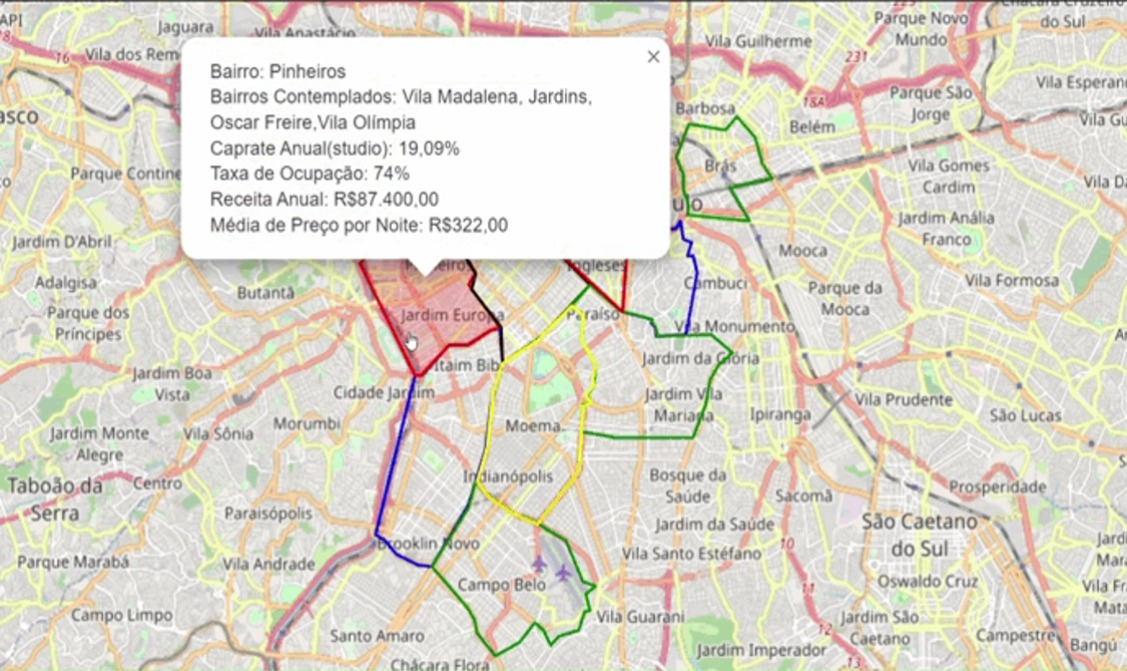
\includegraphics[width = \textwidth]{relatorios/lounge/imagens/1.jpg}
    \end{subfigure}
    \hfill
    \begin{subfigure}{0.49\linewidth}
        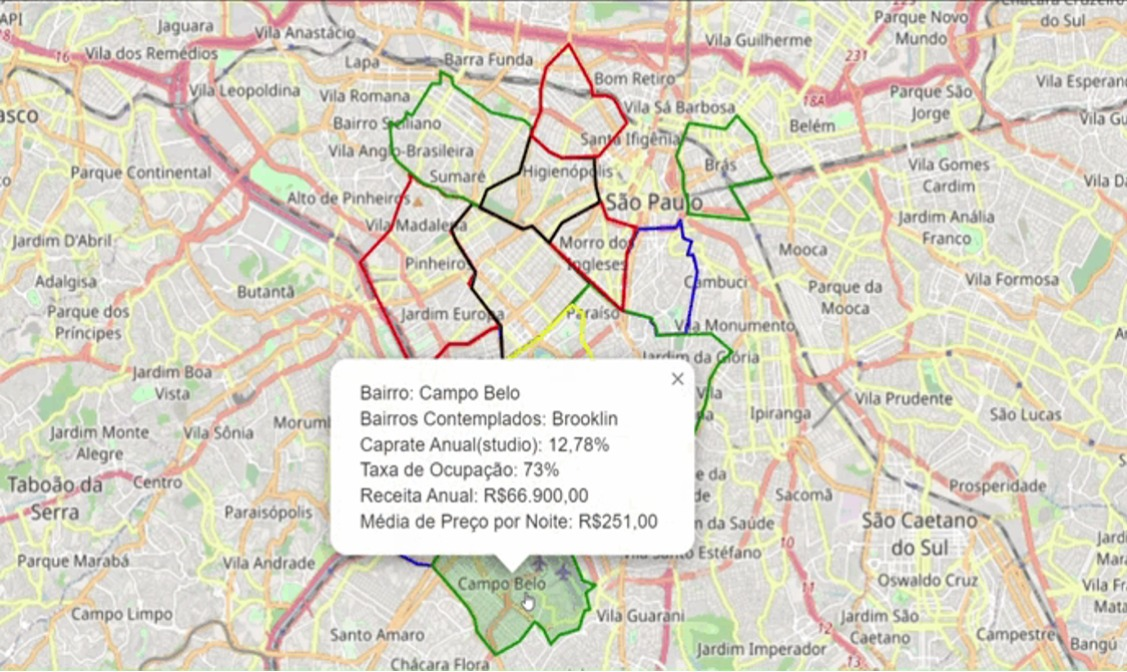
\includegraphics[width = \textwidth]{relatorios/lounge/imagens/2.jpg}
    \end{subfigure}
    \begin{subfigure}{0.49\linewidth}
        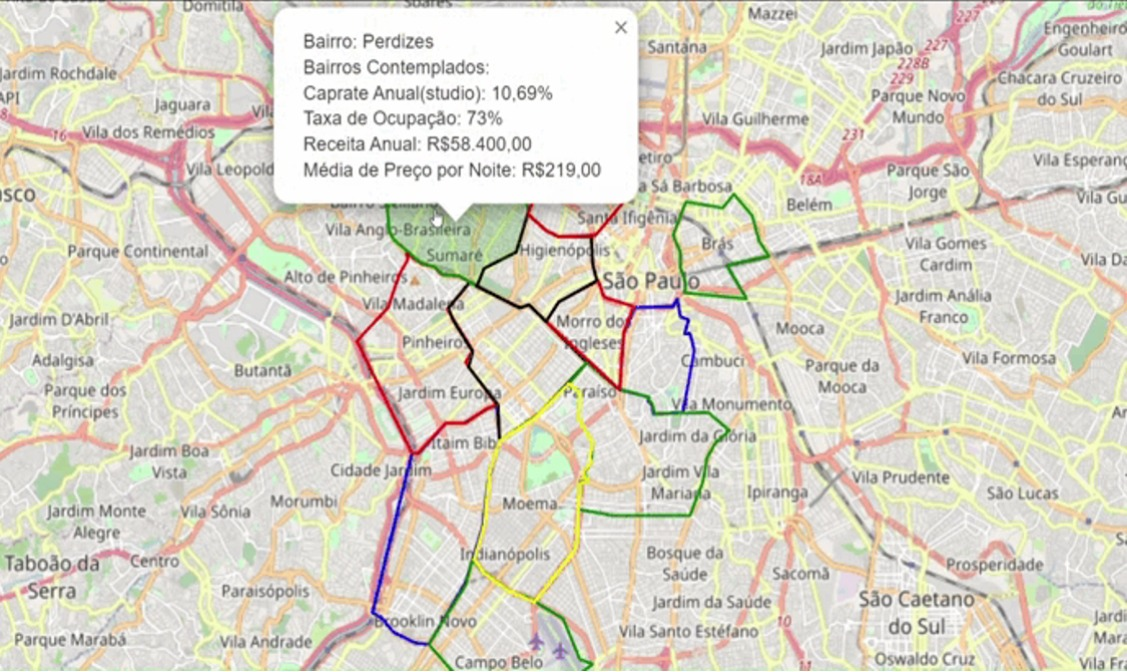
\includegraphics[width = \textwidth]{relatorios/lounge/imagens/3.jpg}
    \end{subfigure}
    \hfill
    \begin{subfigure}{0.49\linewidth}
        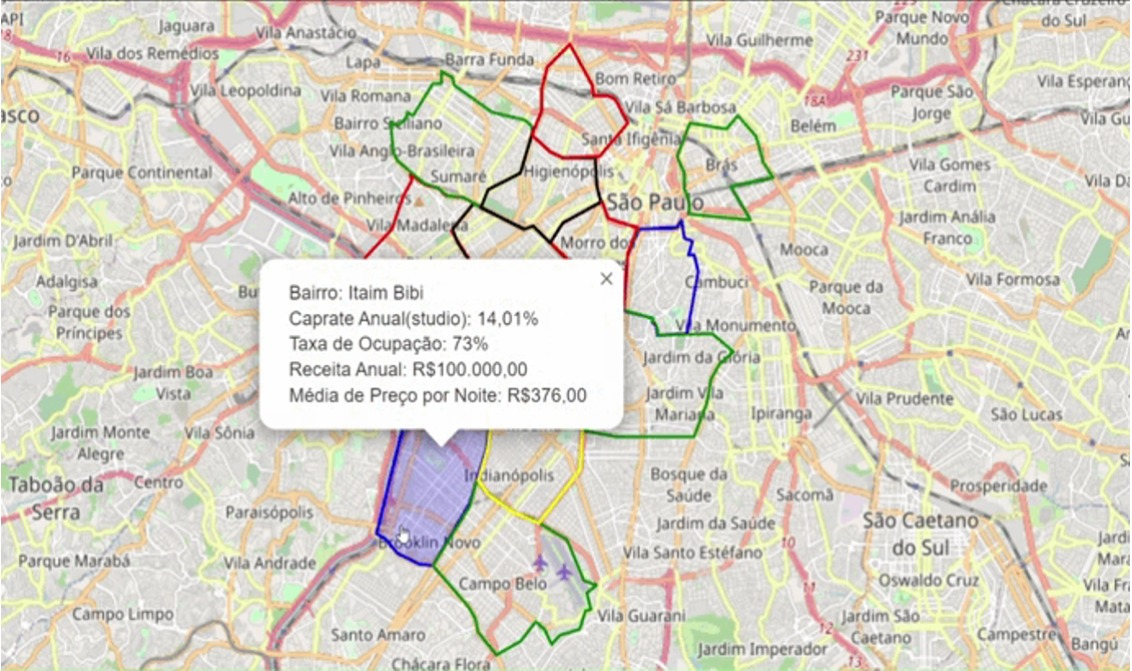
\includegraphics[width = \textwidth]{relatorios/lounge/imagens/4.jpg}
    \end{subfigure}

\end{figure}



\section*{Desafios}

As mudanças de planos em si foi uma dificuldade para nós, afinal quando
ocorreu, o rumo do projeto era completamente diferente e, com o tempo 
passando, a cobrança por resultados começou a ficar mais pesada.

A metodologia para a extração de dados foi u desafiadora também, afinal, 
apesar da biblioteca utilizada ter sido a mesma, os códigos foram bem diferentes, 
pois o Air DNA funciona por assinatura, diferente do Air BNB.

Entretanto, ao longo do semestre, o grupo conseguiu se adaptar bem ao que 
foi proposto e superou as dificuldades, em geral os resultados obtidos foram 
satisfatórios e agora cabe a Lounge 161 utilizar as ferramentas fornecidas pelo 
Insper Data para realizar uma modelagem eficiente tendo em vista o tema central 
do projeto.

\section*{Agradecimentos}

Dentro do Insper Data, recebemos diversas ajudas para desenvolver nosso 
projeto, porém, de forma especial gostaríamos de agradecer ao Presidente Thiago Rocha 
e o Diretor de Projetos André Correa, eles nos deram bons direcionamentos em 
momentos chaves do projeto.

Gostaríamos de agradecer também à Lounge 161 pela confiança depositar em 
nossos esforços para agregar em seus serviços profissionais, de modo especial, Enzo 
Pravatta e Leonardo Franuci que acompanharam o projeto dede o início e mantiveram 
contado e ciência em nossos avanços e desenvolvimentos

\clearpage

\nocite{*}

\printbibliography

\appendix

\end{document}